\documentclass{article}
\usepackage[utf8]{inputenc}
\usepackage[includeheadfoot, margin=1em,headheight=2em]{geometry}
\usepackage{titling}
\geometry{a4paper, left=2cm, right=2cm, top=2cm, bottom=2cm}
\usepackage{graphicx}
\usepackage{float}
\providecommand{\versionnumber}{1.0.0}
\usepackage{enumitem}
\usepackage{array}
\usepackage[italian]{babel}
\newcolumntype{P}[1]{>{\centering\arraybackslash}p{#1}}
\renewcommand{\arraystretch}{1.5} % Default value: 1
\setlength{\droptitle}{-6em}

%font
\usepackage[defaultfam,tabular,lining]{montserrat}
\usepackage[T1]{fontenc}
\renewcommand*\oldstylenums[1]{{\fontfamily{Montserrat-TOsF}\selectfont #1}}

%custom bold 
\usepackage[outline]{contour}
\usepackage{xcolor}
\newcommand{\custombold}{\contour{black}}

%table colors
\usepackage{color, colortbl}
\definecolor{Blue}{rgb}{0.51,0.68,0.79}
\definecolor{LightBlue}{rgb}{0.82,0.87,0.90}
\definecolor{LighterBlue}{rgb}{0.93,0.95,0.96}

%Header
\usepackage{fancyhdr, xcolor}
\pagestyle{fancy}
\let\oldheadrule\headrule% Copy \headrule into \oldheadrule
\renewcommand{\headrule}{\color{Blue}\oldheadrule}% Add colour to \headrule
\renewcommand{\headrulewidth}{0.2em}
\fancyhead[L]{Studio Celonis}
\fancyhead[C]{Samuele Vignotto}
\fancyhead[R]{
\includegraphics[height=1cm]{Logo/Y_LOGO-SOLO.png}}
\setcounter{secnumdepth}{0}

\title{\Huge{\textbf{Microsoft Process Mining}}\vspace{-1em}}
\author{Samuele Vignotto}
\date{}
\begin{document}
\maketitle
\begin{figure}[h]
  \centering
  
\includegraphics[width=6cm, height=6cm]{Logo/Y_LOGO-SOLO.png}
  \label{fig:immagine}
\end{figure}

\newpage
\tableofcontents
\newpage

\section{Introduzione}
Process Mining è un modulo dell'ecosistema Power Automate di Microsoft una soluzione avanzata progettata per aiutare le organizzazioni a migliorare e ottimizzare i propri processi aziendali, sfruttando la potenza dell'analisi dei dati e dell'automazione.

\subsection{Visualizzazione dei processi}
Una delle funzionalità chiave del modulo di Process Mining è la capacità di mappare e visualizzare i processi aziendali così come avvengono realmente. Utilizzando dati storici provenienti da vari sistemi aziendali (ERP, CRM, ecc.), il modulo ricostruisce il flusso di lavoro esistente, permettendo agli utenti di vedere come i processi sono stati eseguiti nel tempo. Questa visualizzazione offre un diagramma chiaro e intuitivo del processo end-to-end, evidenziando le varianti e le deviazioni rispetto al processo ideale.

\subsection{Identificazione delle inefficienze}
Il Process Mining è progettato per identificare colli di bottiglia, ridondanze e altre inefficienze nei processi aziendali. Analizzando i tempi di esecuzione, le deviazioni e i punti di stallo, la soluzione aiuta le aziende a scoprire dove si verificano ritardi o sprechi, offrendo una base solida per intraprendere azioni correttive.

\subsection{Automazione dei processi}
Una volta identificati i punti deboli del processo, Power Automate consente di automatizzare le attività ripetitive e ridondanti. Grazie all'integrazione con la suite Power Automate, è possibile creare flussi di lavoro automatizzati che riducono l'intervento manuale, migliorano l'efficienza e riducono il rischio di errori umani.

\subsection{Monitoraggio continuo e ottimizzazione}
Il modulo di Process Mining non si limita ad analizzare i processi una tantum, ma permette anche un monitoraggio continuo. Le aziende possono impostare alert e notifiche per monitorare le performance dei processi in tempo reale e intervenire prontamente in caso di anomalie. Questo monitoraggio continuo supporta un miglioramento continuo dei processi, permettendo alle organizzazioni di adattarsi rapidamente ai cambiamenti del mercato e alle esigenze dei clienti.

\subsection{Analisi predittiva e simulazioni}
Grazie all'analisi dei dati storici e all'uso di algoritmi avanzati, Power Automate Process Mining può anche prevedere l'andamento futuro dei processi. Le funzionalità di simulazione permettono agli utenti di testare diversi scenari e valutare l'impatto di eventuali modifiche, prima di implementarle realmente. Questo approccio proattivo consente di pianificare con maggiore precisione e di prendere decisioni informate per migliorare l'efficienza operativa.

\subsection{Integrazione con strumenti Microsoft}
Un altro vantaggio significativo del modulo Process Mining è la sua perfetta integrazione con altri strumenti e servizi Microsoft, come Power BI per l'analisi dei dati e la visualizzazione avanzata, e Dynamics 365 per la gestione delle operazioni aziendali. Questa integrazione consente di sfruttare al massimo l'ecosistema Microsoft, offrendo una visione unificata e completa delle operazioni aziendali.

\section{Formati di File Accettati}

\subsection{CSV (Comma-Separated Values)}
Il formato CSV è uno dei più comuni per l'importazione di log degli eventi. I file CSV possono essere caricati direttamente tramite \textit{OneDrive for Business} o altre piattaforme di archiviazione supportate.

\subsection{Excel (XLSX)}
I file Excel sono supportati, permettendo l'importazione di dati strutturati in fogli di calcolo. Questo è utile quando i dati sono già organizzati in formato tabellare e contengono più fogli con informazioni correlate.

\subsection{JSON (JavaScript Object Notation)}
I file JSON possono essere utilizzati per strutturare dati complessi, specialmente quando si tratta di dati gerarchici o di oggetti complessi, che devono essere analizzati in modo approfondito.

\subsection{Database relazionali (SQL Server, MySQL, PostgreSQL)}
È possibile collegarsi direttamente a database relazionali per importare dati in tempo reale. Questo è particolarmente utile per aziende che hanno grandi volumi di dati archiviati in database come SQL Server o PostgreSQL.

\subsection{Dataverse}
Microsoft Dataverse, parte di Power Platform, è supportato per gestire dati all'interno di ambienti Microsoft 365 e Dynamics 365. Questa piattaforma offre una gestione dei dati altamente scalabile e integrata con altre applicazioni Microsoft.

\section{Fonti di Dati Supportate}

\subsection{Connettori per Applicazioni SaaS}
Sono disponibili connettori diretti per applicazioni enterprise come \textit{SAP, Salesforce} e \textit{Dynamics 365}, permettendo di estrarre i log degli eventi e altri dati rilevanti direttamente dai sistemi SaaS.

\subsection{Servizi di Archiviazione Cloud}
È possibile collegarsi a servizi di archiviazione cloud come \textit{OneDrive, SharePoint, Google Drive} per importare file in vari formati, tra cui CSV, Excel o JSON.

\subsection{Power Query}
\textit{Power Query} è uno strumento integrato in Power BI che consente di connettersi a una vasta gamma di fonti di dati, compresi servizi web, API e database on-premise, facilitando la trasformazione e l'importazione dei dati necessari per il process mining.

\subsection{Servizi Web e API}
È possibile importare dati da servizi web RESTful e altre API, consentendo di integrare flussi di dati in tempo reale per l'analisi dei processi.

\subsection{Altri Servizi di Business Intelligence}
Strumenti di BI come \textit{Azure Data Lake, Azure SQL Database} e \textit{Google BigQuery} sono supportati, permettendo l'integrazione con grandi dataset per analisi approfondite.


\section{Funzionalità}
\subsection{Process map}
La sezione "Process map" dello strumento di process mining di Microsoft rappresenta un aspetto centrale dell'analisi dei processi aziendali, consentendo di visualizzare e comprendere in modo chiaro ed efficace il flusso delle attività all'interno di un'organizzazione. Questa sezione si distingue per la sua capacità di trasformare dati complessi in rappresentazioni visive intuitive, offrendo così una comprensione immediata delle dinamiche operative.\\
Ogni attività svolta all'interno del flusso di lavoro viene tracciata e rappresentata come un nodo su una mappa, collegato da frecce che indicano la sequenza e la direzione delle operazioni. Questa rappresentazione non solo illustra il percorso ideale delle operazioni, ma mette anche in evidenza tutte le deviazioni e le varianti che possono verificarsi.\\
Un altro aspetto fondamentale della "Process map" è la capacità di analizzare la frequenza e la durata delle diverse attività. Ogni percorso e nodo può essere arricchito con informazioni quantitative, come il numero di volte in cui un determinato passaggio è stato eseguito e il tempo medio impiegato per completarlo. Questo permette agli utenti di identificare rapidamente le aree critiche o i colli di bottiglia, dove il processo potrebbe essere rallentato o dove si verificano la maggior parte degli errori.\\
La "Process map" supporta anche la personalizzazione e il filtraggio dei dati. Gli utenti possono selezionare specifiche porzioni del processo, focalizzandosi su un periodo temporale particolare o su un sottoinsieme di casi che soddisfano criteri definiti. Questo livello di dettaglio consente di esaminare i processi con un'ottica precisa, rendendo possibile l’individuazione di problemi specifici e l’analisi delle loro cause radice.

\subsection{Process animation}
Attraverso l'animazione dei processi, gli utenti possono vedere in tempo reale come le attività vengono eseguite, con ogni evento che si manifesta visivamente sulla mappa del processo.\\
La caratteristica distintiva della "Process animation" è la sua capacità di riprodurre il flusso delle operazioni nel tempo, come se si stesse guardando una simulazione del processo stesso. Ogni transizione tra le attività viene visualizzata con una progressione fluida, mostrando chiaramente come le operazioni si susseguono. Questo consente agli utenti di cogliere rapidamente l’ordine degli eventi e di comprendere come le diverse parti del processo interagiscono tra loro.\\
Gli utenti possono accelerare o rallentare l’animazione per analizzare con precisione le parti del processo che risultano più critiche o complesse. Ad esempio, è possibile rallentare la riproduzione per osservare da vicino i passaggi in cui si verificano colli di bottiglia, oppure accelerare per avere una visione d'insieme del processo nel suo complesso.\\
Durante l’animazione, gli utenti possono osservare come si accumulano le attività in determinati punti del processo, rivelando potenziali inefficienze o aree di sovraccarico. Inoltre, la possibilità di visualizzare le varianti del processo in movimento permette di confrontare in tempo reale diversi flussi di lavoro, individuando immediatamente le differenze e comprendendo meglio le cause delle variazioni.\\
Un ulteriore vantaggio della funzionalità di animazione è la capacità di enfatizzare eventi specifici, come ritardi o errori. Questi possono essere rappresentati con colori o segnali distintivi durante l'animazione, rendendo immediatamente visibili i problemi che potrebbero richiedere un intervento.\\

\subsection{Statistics}
Questa sezione è progettata per fornire dati precisi e utili che consentono di approfondire la comprensione del funzionamento dei processi e identificare opportunità di miglioramento.\\
Gli utenti possono accedere a statistiche che descrivono il numero di volte in cui un'attività specifica è stata eseguita, il tempo medio impiegato per ciascun passaggio, e la variazione di questi tempi all'interno di diversi intervalli temporali o per diversi casi. Questo permette una visione chiara non solo dell'efficienza del processo nel suo complesso, ma anche delle prestazioni di singole attività.\\
Un aspetto fondamentale delle statistiche offerte è la possibilità di eseguire confronti tra diverse versioni o varianti del processo. Ad esempio, gli utenti possono analizzare come una specifica attività si comporta in differenti contesti, come in diverse sedi aziendali o sotto condizioni operative diverse. Questo confronto aiuta a identificare le migliori pratiche o a individuare aree in cui determinati cambiamenti possono avere un impatto significativo sulle performance complessive.\\
Inoltre, la funzionalità "Statistics" offre strumenti per segmentare i dati, permettendo di filtrare e analizzare le informazioni per sottogruppi specifici, come particolari clienti, tipologie di ordini, o periodi temporali.\\
Infine, la rappresentazione visiva dei dati statistici è curata in modo tale da facilitare l'interpretazione. Grafici, istogrammi, e tabelle riassuntive sono utilizzati per visualizzare chiaramente le informazioni, rendendo immediatamente evidenti le distribuzioni dei dati e le relazioni tra le diverse metriche.

\subsection{Root cause analysis}
Al centro della "Root cause analysis" c'è la capacità di analizzare sistematicamente le deviazioni o i problemi osservati all'interno di un processo, risalendo alle origini di questi problemi attraverso una serie di strumenti analitici avanzati. Quando viene rilevato un comportamento anomalo nel processo, come un ritardo significativo, un errore frequente, o una deviazione dalle procedure standard, questa funzionalità permette di esplorare le varie dimensioni del problema, scomponendo il processo per identificare i fattori specifici che contribuiscono a tale anomalia.\\
Uno degli aspetti più importanti della "Root cause analysis" è la sua capacità di incrociare e analizzare variabili multiple contemporaneamente. Ad esempio, se un processo presenta ritardi sistematici, lo strumento può esaminare diverse dimensioni come il tempo, le risorse coinvolte, i tipi di casi, e le condizioni operative per individuare correlazioni significative. Questo permette di identificare non solo che un problema esiste, ma anche quali combinazioni di fattori sono più probabilmente alla base di quel problema.\\
La funzionalità si avvale anche di tecniche avanzate di data mining e machine learning per identificare pattern nascosti nei dati che potrebbero non essere immediatamente evidenti attraverso un'analisi superficiale. Ad esempio, lo strumento può individuare correlazioni tra una specifica configurazione di risorse e l'insorgenza di errori, o tra un particolare percorso di processo e l'aumento dei tempi di attesa. Questi insight sono cruciali per capire le dinamiche sottostanti che influenzano le performance del processo.\\
Inoltre, la "Root cause analysis" è progettata per essere altamente interattiva e visiva. Gli utenti possono esplorare i dati attraverso visualizzazioni dinamiche che evidenziano le relazioni causali tra diverse variabili. La capacità di visualizzare immediatamente l'impatto di diversi fattori aiuta a guidare il processo decisionale e a determinare quali azioni correttive potrebbero avere l'effetto più significativo.\\
Infine, la funzionalità "Root cause analysis" supporta un processo decisionale informato e data-driven. Una volta identificate le cause principali di un problema, lo strumento può essere utilizzato per simulare l'effetto di potenziali interventi correttivi, permettendo di valutare in anticipo l'efficacia di diverse soluzioni.

\subsection{Variants}
Al cuore della funzionalità "Variants" vi è la capacità di mappare e visualizzare tutte le possibili sequenze di attività che compongono un processo. In molti contesti aziendali, un processo non segue sempre un percorso lineare e standardizzato; possono esistere molte varianti basate su fattori come eccezioni, deviazioni o personalizzazioni per specifici clienti o ordini. Questa funzionalità consente di identificare e quantificare queste varianti, mostrando chiaramente quante volte e in quali circostanze ciascuna variante si verifica.\\
La visualizzazione delle varianti è una delle caratteristiche più potenti di questa funzionalità. Gli utenti possono vedere graficamente come il processo si dirama in vari percorsi, con ciascuna variante rappresentata come un flusso distinto. Questa visualizzazione permette di cogliere immediatamente quali percorsi sono più comuni, quali sono meno frequenti e, soprattutto, dove si manifestano le deviazioni rispetto al processo ideale o previsto.\\
Un altro aspetto chiave della funzionalità "Variants" è la possibilità di confrontare le prestazioni tra diverse varianti. Gli utenti possono analizzare come la durata, i costi, o la qualità del processo cambiano a seconda della variante presa in esame. Ad esempio, può emergere che una particolare variante, pur essendo meno comune, comporta tempi di completamento significativamente più rapidi o, al contrario, che una variante più frequente è associata a un numero maggiore di errori o ritardi. Questo tipo di analisi è essenziale per identificare opportunità di standardizzazione o per focalizzare gli sforzi di miglioramento su varianti che contribuiscono maggiormente alle inefficienze.\\
La funzionalità "Variants" consente anche di filtrare e segmentare le varianti in base a criteri specifici. Gli utenti possono esplorare le varianti in base a fattori come il cliente, il tipo di prodotto, il periodo temporale o altre dimensioni rilevanti. Questo livello di dettaglio è fondamentale per comprendere non solo quali varianti esistono, ma anche perché si verificano, permettendo di individuare le cause sottostanti alle differenze operative.

\subsection{Process compare}
Questa funzionalità è particolarmente utile per le organizzazioni che desiderano confrontare l'efficienza, la conformità, e le performance operative di diversi flussi di lavoro, sia all'interno della stessa unità aziendale che tra unità diverse.\\
Questa comparazione avviene attraverso una rappresentazione grafica che mette in evidenza i punti in cui i processi divergono, non solo in termini di sequenza delle attività, ma anche in base a metriche chiave come la durata, i costi, e la frequenza delle varie fasi del processo. In questo modo, è possibile vedere a colpo d’occhio come i processi si comportano in diversi scenari o sotto condizioni operative differenti.\\
Quando si confrontano due processi, è possibile individuare esattamente dove e come differiscono, e quale impatto queste differenze hanno sulle performance complessive. Per esempio, se un processo in una sede aziendale richiede significativamente più tempo rispetto a un'altra sede, lo strumento consente di individuare le specifiche attività che causano questi ritardi e di comprendere le ragioni alla base di tali differenze.\\
La funzionalità permette anche di analizzare le best practice all'interno dell’organizzazione. Confrontando le performance di diverse varianti del processo, gli utenti possono identificare quali configurazioni operative portano ai risultati migliori. Queste informazioni sono preziose per standardizzare le procedure e implementare le pratiche più efficienti su scala più ampia all'interno dell'organizzazione.\\
Inoltre, "Process Compare" offre strumenti di filtraggio avanzati, che consentono di limitare l'analisi a determinati intervalli temporali, specifiche risorse, o particolari gruppi di casi. Questo livello di dettaglio è essenziale per capire le differenze nei processi sotto differenti condizioni operative, come ad esempio in periodi di picco della domanda o quando vengono impiegate risorse diverse. Tale granularità permette un'analisi estremamente mirata, facilitando l'individuazione delle cause di eventuali inefficienze o problemi specifici.

\section{Integrazioni con Strumenti Microsoft}

\subsection{Microsoft Power BI}
Microsoft Power BI è strettamente integrato con lo strumento di process mining. Power BI consente di creare report visivi dettagliati che aiutano a identificare colli di bottiglia e a migliorare i processi aziendali. L'integrazione con Power BI permette di trasformare i dati di process mining in insight azionabili, utilizzando dashboard interattivi e report personalizzabili.

\subsection{Microsoft Power Automate}
Power Automate è la piattaforma centrale per eseguire process mining all'interno dell'ecosistema Microsoft. Con Power Automate, è possibile automatizzare i flussi di lavoro basati su dati di process mining, collegando diverse applicazioni e servizi per ottimizzare i processi aziendali in tempo reale.

\subsection{Microsoft Dynamics 365}
Dynamics 365 si integra perfettamente con lo strumento di process mining, permettendo di analizzare i processi all'interno dei moduli ERP e CRM. Questa integrazione consente di ottenere una visione completa dei processi aziendali, dalla gestione delle relazioni con i clienti fino alla catena di fornitura.

\subsection{Microsoft Dataverse}
Dataverse fornisce un'infrastruttura dati centralizzata che è altamente integrata con lo strumento di process mining. Questa integrazione permette di gestire i dati aziendali in modo centralizzato e di utilizzarli per analisi avanzate dei processi, facilitando la gestione e la condivisione dei dati tra diverse applicazioni all'interno della piattaforma Microsoft Power.

\subsection{Microsoft Azure}
Azure offre una serie di servizi che possono essere utilizzati in combinazione con lo strumento di process mining. Azure Data Lake e Azure SQL Database sono particolarmente utili per l'archiviazione e l'elaborazione di grandi volumi di dati, che possono poi essere analizzati tramite Power BI e Power Automate.

\subsection{Microsoft SharePoint}
SharePoint si integra con lo strumento di process mining, consentendo di accedere e condividere documenti e dati utilizzati nei processi di analisi. L'integrazione con SharePoint facilita la collaborazione tra i team e la condivisione dei risultati delle analisi dei processi.

\subsection{Microsoft Teams}
Teams può essere utilizzato in combinazione con lo strumento di process mining per facilitare la collaborazione e la comunicazione tra i membri del team. I risultati delle analisi possono essere condivisi direttamente in Teams, permettendo ai team di discutere e prendere decisioni basate sui dati in modo più efficiente.


\section{Implementazioni pratiche: simulazioni}
\subsection{Prima simulazione}
\subsubsection{Struttura del file CSV}
Il file CSV con i dati simulati contiene informazioni riguardanti le attività di una ditta che riceve prodotti da un'azienda, li vende online e li spedisce ai clienti. La struttura del file è la seguente:
\begin{itemize}
    \item \custombold{activity\_id}: identificativo univoco per ogni attività;
    \item \custombold{activity}: nome dell'attività svolta;
    \item \custombold{timestamp}: data e ora in cui l'attività è stata svolta;
    \item \custombold{product\_id}: identificativo del prodotto coinvolto nell'attività.
\end{itemize}
Esempio di contenuto del file CSV:
\begin{table}[htbp]
    \centering
    \begin{tabular}{|c|c|c|c|}
        \hline
        \textbf{activity\_id} & \textbf{activity} & \textbf{timestamp} & \textbf{product\_id} \\
        \hline
        1 & Receive Goods & 2023-08-02 18:20:10.465195 & 1 \\
        \hline
        2 & Quality Check & 2023-12-03 13:30:22.465195 & 1 \\
        \hline
        3 & Store in Warehouse & 2024-03-09 18:03:55.465195 & 1 \\
        \hline
        4 & Pick for Order & 2024-03-15 02:03:15.465195 & 1 \\
        \hline
        5 & Order Cancellation & 2024-05-29 08:01:26.465195 & 1 \\
        \hline
    \end{tabular}
    \caption{Activity Log}
    \label{tab:activity_log}
\end{table}
\subsubsection{Regole di simulazione dei dati}
I dati simulati sono stati generati seguendo determinate regole per garantire la coerenza temporale e la rappresentazione realistica dei processi aziendali. Le regole principali sono:
\begin{itemize}
    \item \custombold{Coerenza dei Timestamps}: I timestamp delle attività devono essere coerenti. Ad esempio, il timestamp della spedizione al cliente non può essere precedente al timestamp dell'ordine.
    \item \custombold{Cicli di attività possibili}:
    \begin{itemize}
        \item \custombold{Ciclo 1}: Receive Goods -> Quality Check -> Store in Warehouse
        \item \custombold{Ciclo 2}: Receive Goods -> Quality Check -> Store in Warehouse -> Pick for Order -> Order Cancellation
        \item \custombold{Ciclo 3}: Receive Goods -> Quality Check -> Store in Warehouse -> Pick for Order -> Receive Payment -> Pack for Shipment -> Ship to Customer -> Customer Receive Goods
        \item \custombold{Ciclo 4}: Receive Goods -> Quality Check -> Store in Warehouse -> Pick for Order -> Receive Payment -> Pack for Shipment -> Ship to Customer -> Customer Receive Goods -> Customer Feedback
        \item \custombold{Ciclo 5}: Receive Goods -> Quality Check -> Store in Warehouse -> Pick for Order -> Receive Payment -> Pack for Shipment -> Ship to Customer -> Customer Receive Goods -> Customer Feedback -> Return Processing
    \end{itemize}
\end{itemize}

\subsubsection{Process map}
\begin{figure}[H]
    \centering
    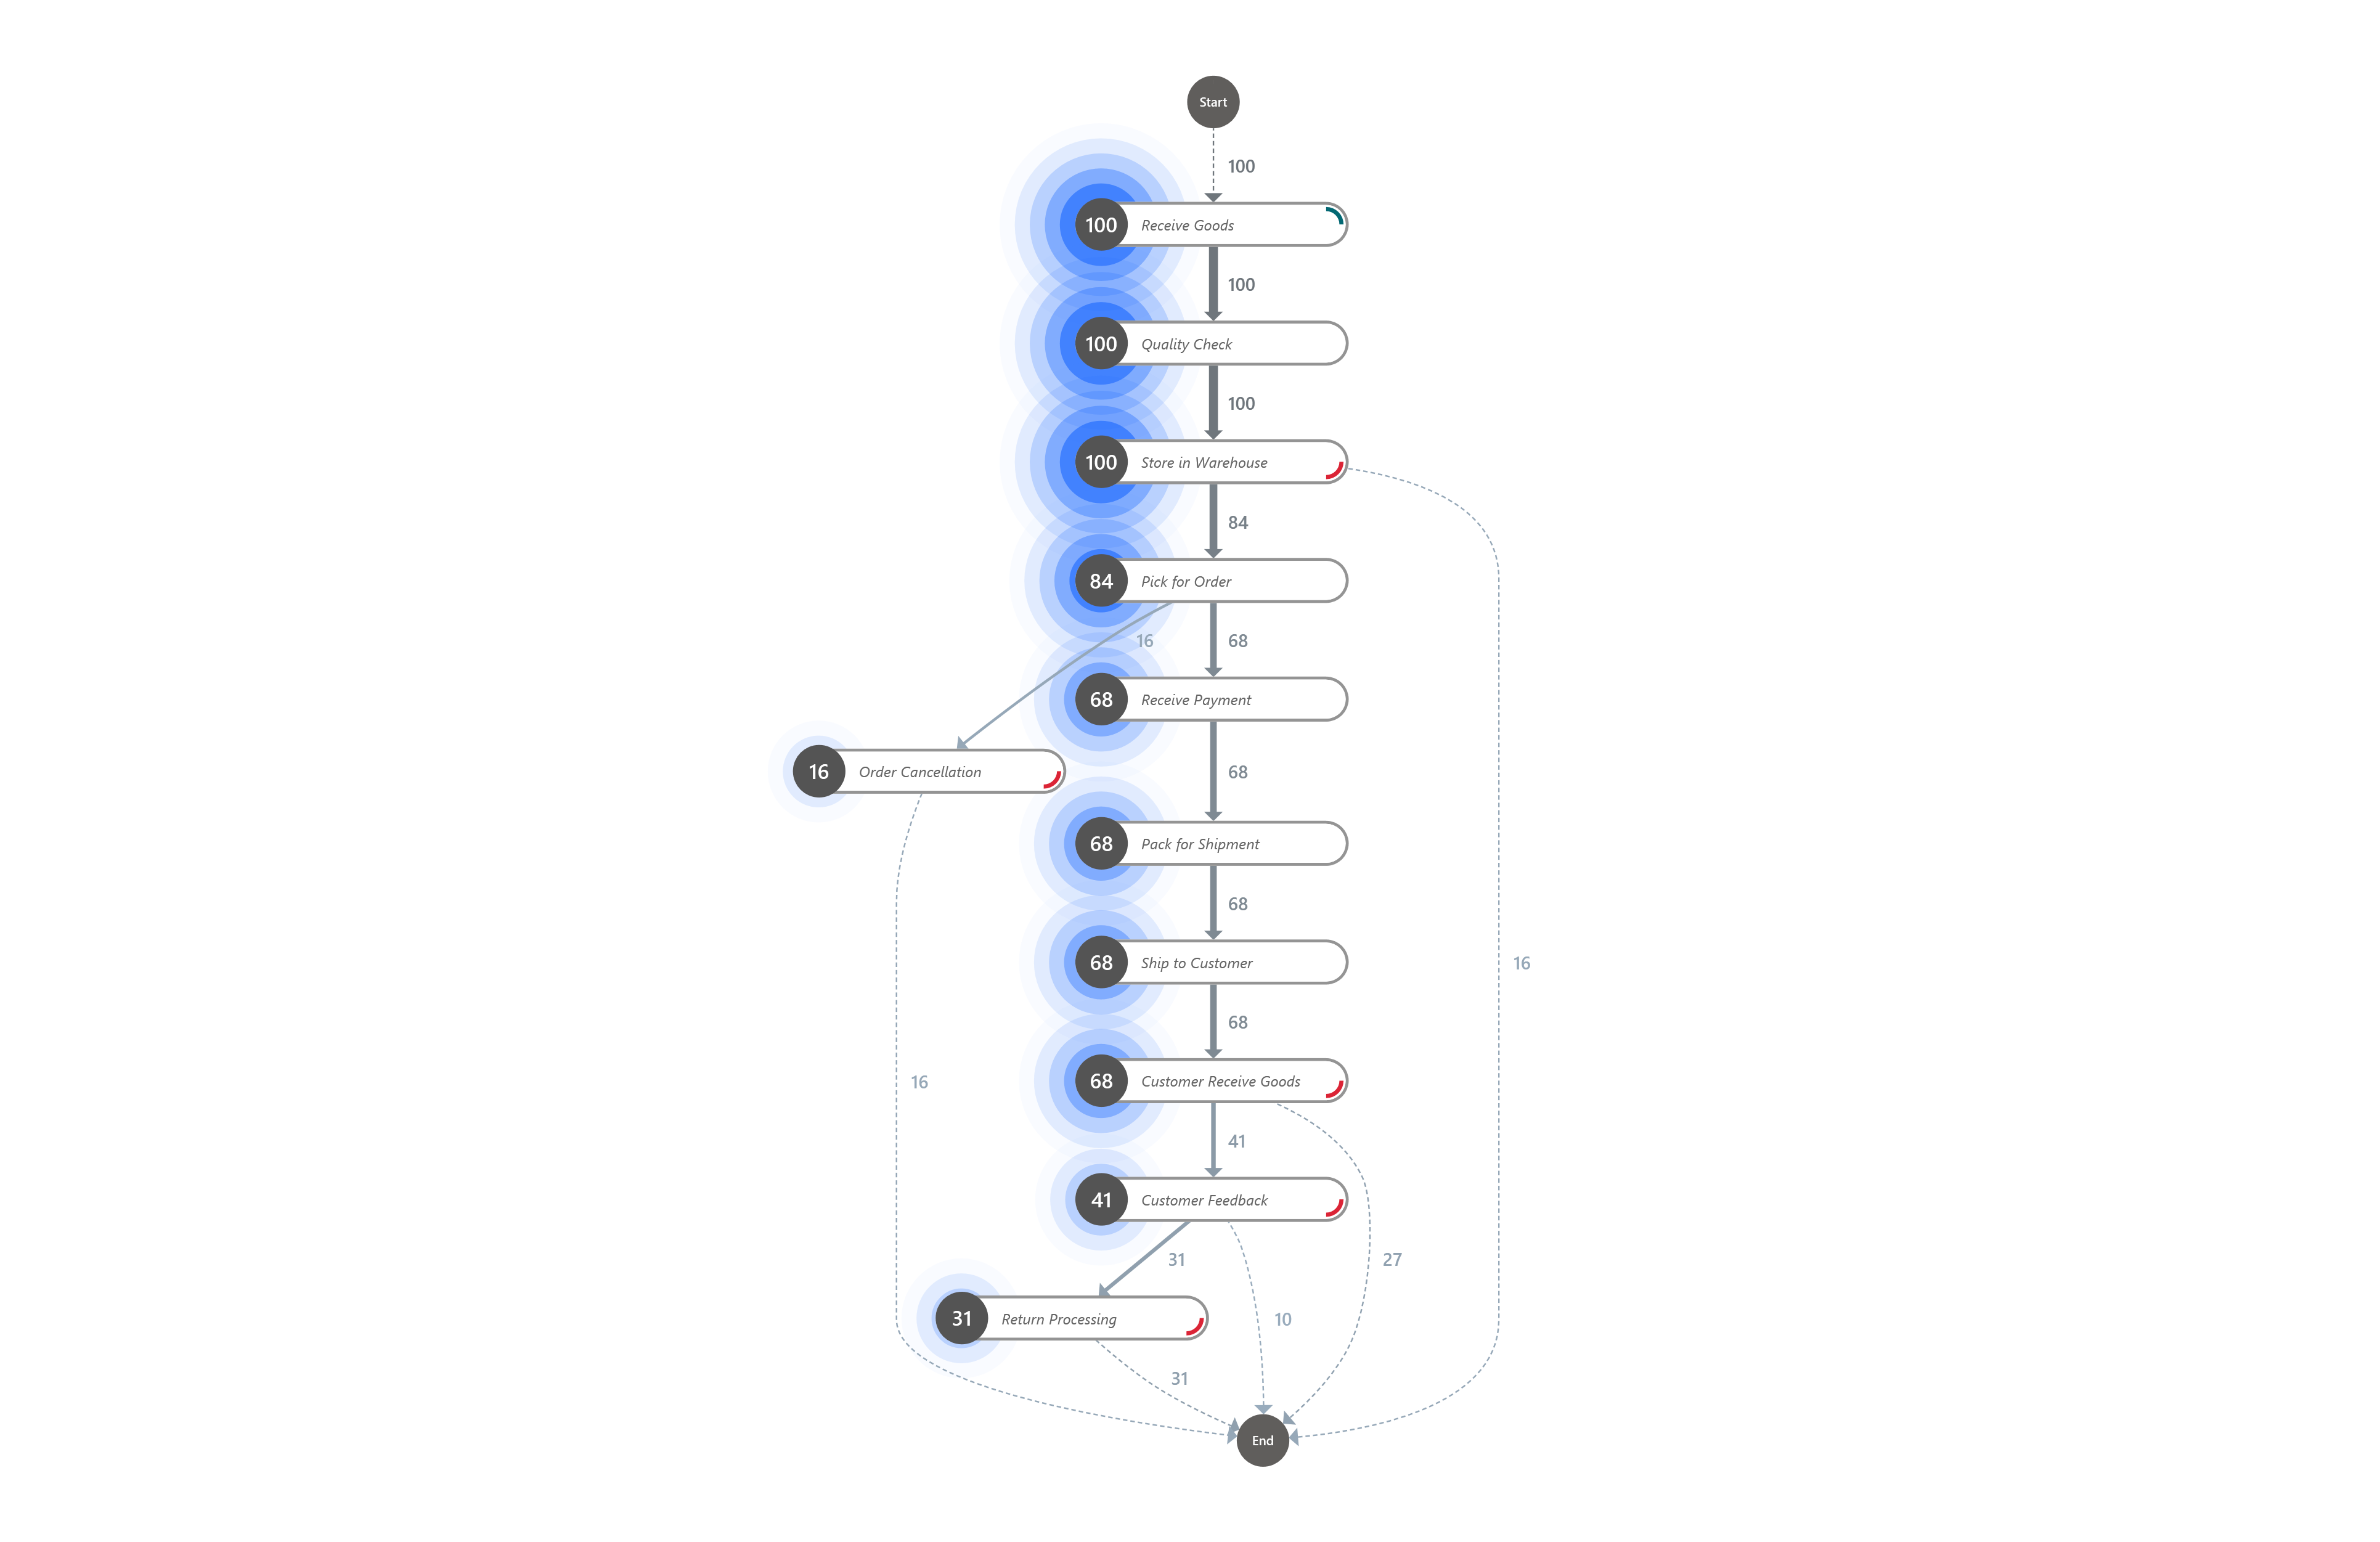
\includegraphics[width=\textwidth]{imgMicrosoft/PrimaSimulazione/ProcessMapSimulazione1.png}
    \caption{Mappa del processo}
    \label{fig:process-map}
\end{figure}
La mappa di processo offre una chiara visualizzazione dei vari passaggi e delle possibili transizioni tra le attività. Le percentuali di completamento per ciascuna attività sono rappresentate dalle dimensioni delle bolle, mentre le connessioni tra di esse indicano la frequenza delle transizioni.\\
Ad esempio, si osserva che il passaggio tra le attività "Receive Goods" e "Store in Warehouse" è molto comune, suggerendo che questo segmento del processo è una routine consolidata. D'altra parte, il passaggio verso la "Order Cancellation" è meno frequente, indicando che le cancellazioni degli ordini avvengono in una minoranza di casi, ma sono comunque un aspetto previsto del flusso di lavoro.\\
La visualizzazione di queste dinamiche offre importanti spunti sull'efficienza del processo. Le aree con percentuali di transizione più basse o con deviazioni significative possono rappresentare punti critici o meno efficienti che potrebbero beneficiare di ulteriori analisi e miglioramenti.\\
La mappa di processo è coerente con le regole di simulazione dei dati e riflette in modo accurato e realistico le operazioni aziendali. La struttura del flusso di lavoro è logica e ben organizzata, rispettando la coerenza temporale tra le attività. Inoltre, la mappa fornisce una chiara rappresentazione delle diverse varianti del processo, permettendo di identificare facilmente i punti di forza e le aree di miglioramento.

\subsubsection{Statistics case overview}
\begin{figure}[H]
    \centering
    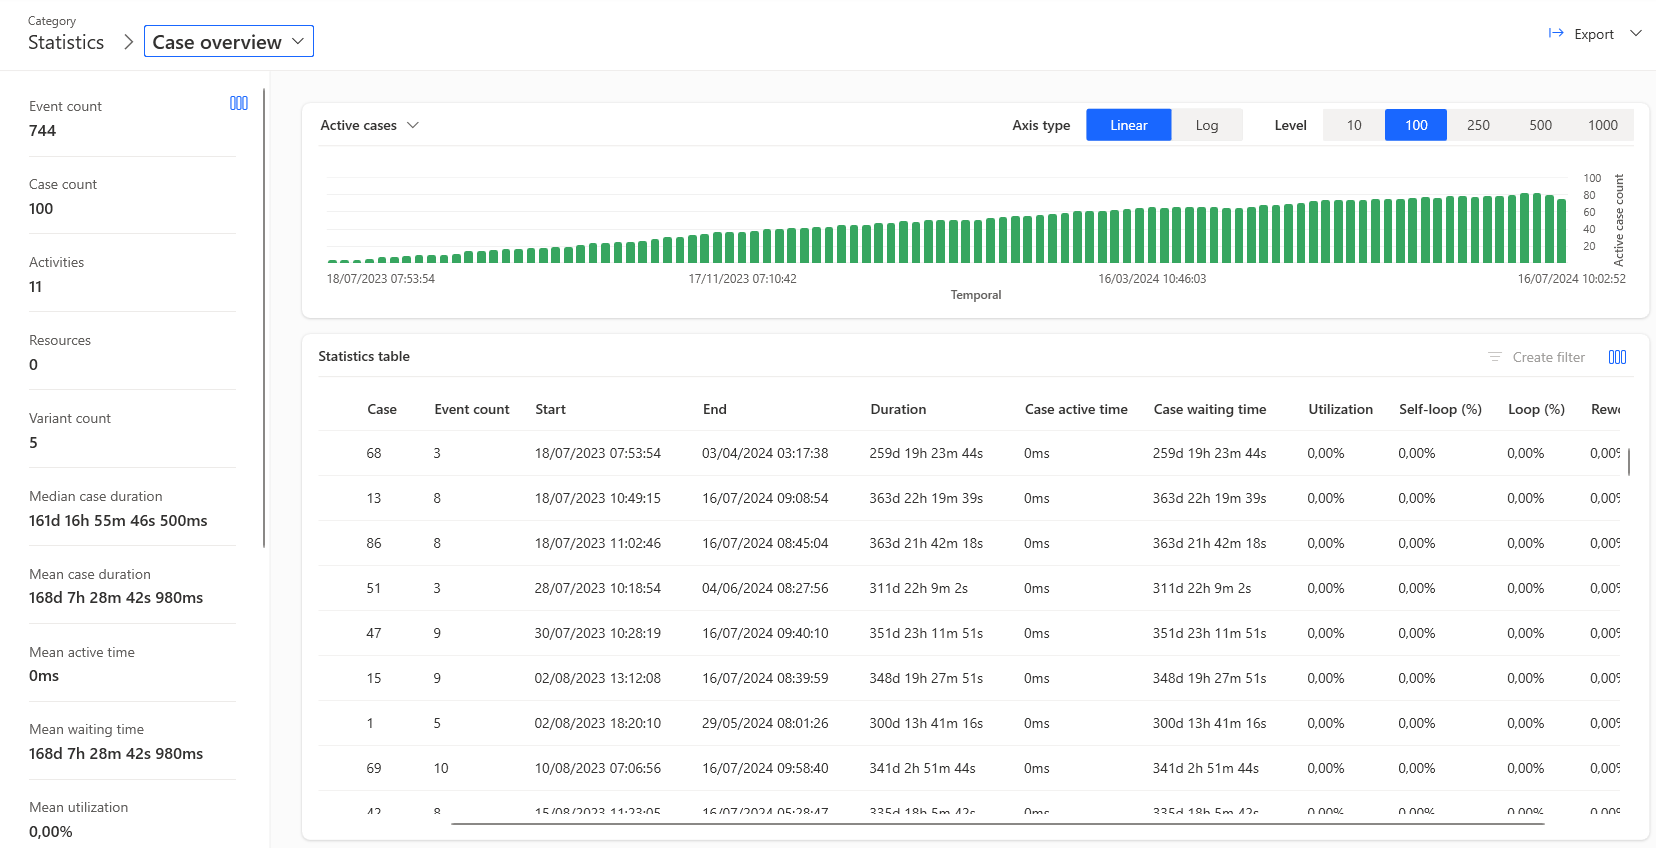
\includegraphics[width=\textwidth]{imgMicrosoft/PrimaSimulazione/StatisticsCaseOverviewSimulazione1.png}
    \caption{Panoramica dei casi}
    \label{fig:statistics-case-overview}
\end{figure}
La schermata di panoramica dei casi fornisce un'analisi dettagliata del comportamento dei casi all'interno del processo simulato. Questa schermata esamina vari aspetti, come la durata totale dei casi, il numero di eventi per caso, il tempo di attesa e l'utilizzo. L'obiettivo di questa analisi è comprendere meglio la distribuzione temporale dei casi, identificare eventuali colli di bottiglia e valutare l'efficienza complessiva del processo.\\
Il numero totale di eventi registrati è 744, distribuiti su 100 casi, con un totale di 11 attività coinvolte nel processo. La schermata evidenzia anche che ci sono 5 varianti di processo, indicando che non tutti i casi seguono esattamente lo stesso percorso all'interno del flusso di lavoro.\\
La durata mediana dei casi è di 161 giorni, 16 ore, 55 minuti e 46 secondi, con una durata media leggermente superiore di 168 giorni, 7 ore, 28 minuti e 42 secondi. Questo suggerisce una leggera asimmetria nei dati, con alcuni casi che hanno una durata significativamente superiore alla media. La distribuzione delle durate dei casi può fornire indicazioni utili su quali varianti del processo siano più lunghe e se queste durate siano dovute a specifiche attività o ritardi.\\
I tempi di attesa medi coincidono esattamente con la durata media dei casi, il che indica che non c'è tempo di attività effettiva registrato all'interno dei casi; tutti i casi hanno un "active time" riportato come 0 ms. Questo potrebbe indicare che, nella simulazione, il tempo è stato considerato solo in termini di durata totale del processo e non è stato possibile determinare quanto tempo è stato effettivamente dedicato alle attività specifiche all'interno di ogni caso.\\
La visualizzazione degli "Active cases" mostra un progressivo aumento nel numero di casi attivi nel tempo. Questo potrebbe suggerire un processo che accumula casi nel tempo, con nuovi casi che entrano nel sistema mentre quelli precedenti non sono ancora completati. Questo tipo di distribuzione può essere indicativo di un backlog nel processo o di un ciclo di lavoro che si estende su lunghi periodi.\\
L'analisi delle varianti dei casi rivela una certa variabilità nei percorsi seguiti. Ad esempio, nella tabella delle statistiche, si può osservare che i casi con ID 13 e 86, che seguono varianti diverse, hanno un numero di eventi superiore rispetto ad altri casi, il che potrebbe indicare percorsi più complessi o che coinvolgono più attività.\\
La schermata di panoramica dei casi fornisce una visione esaustiva della durata e della distribuzione dei casi all'interno del processo. La durata relativamente lunga dei casi e la coincidenza dei tempi di attesa con la durata totale suggeriscono che i casi sono stati simulati con un approccio che considera solo la durata complessiva del processo, senza dettagli sulle attività intermedie.\\
La variabilità nelle durate dei casi e il numero di varianti indicano un processo con una certa flessibilità e complessità, dove non tutti i casi seguono lo stesso percorso. Questo potrebbe offrire spunti per ulteriori analisi, come l'identificazione di colli di bottiglia o l'ottimizzazione dei tempi di attesa.

\subsubsection{Statistics activity}
\begin{figure}[H]
    \centering
    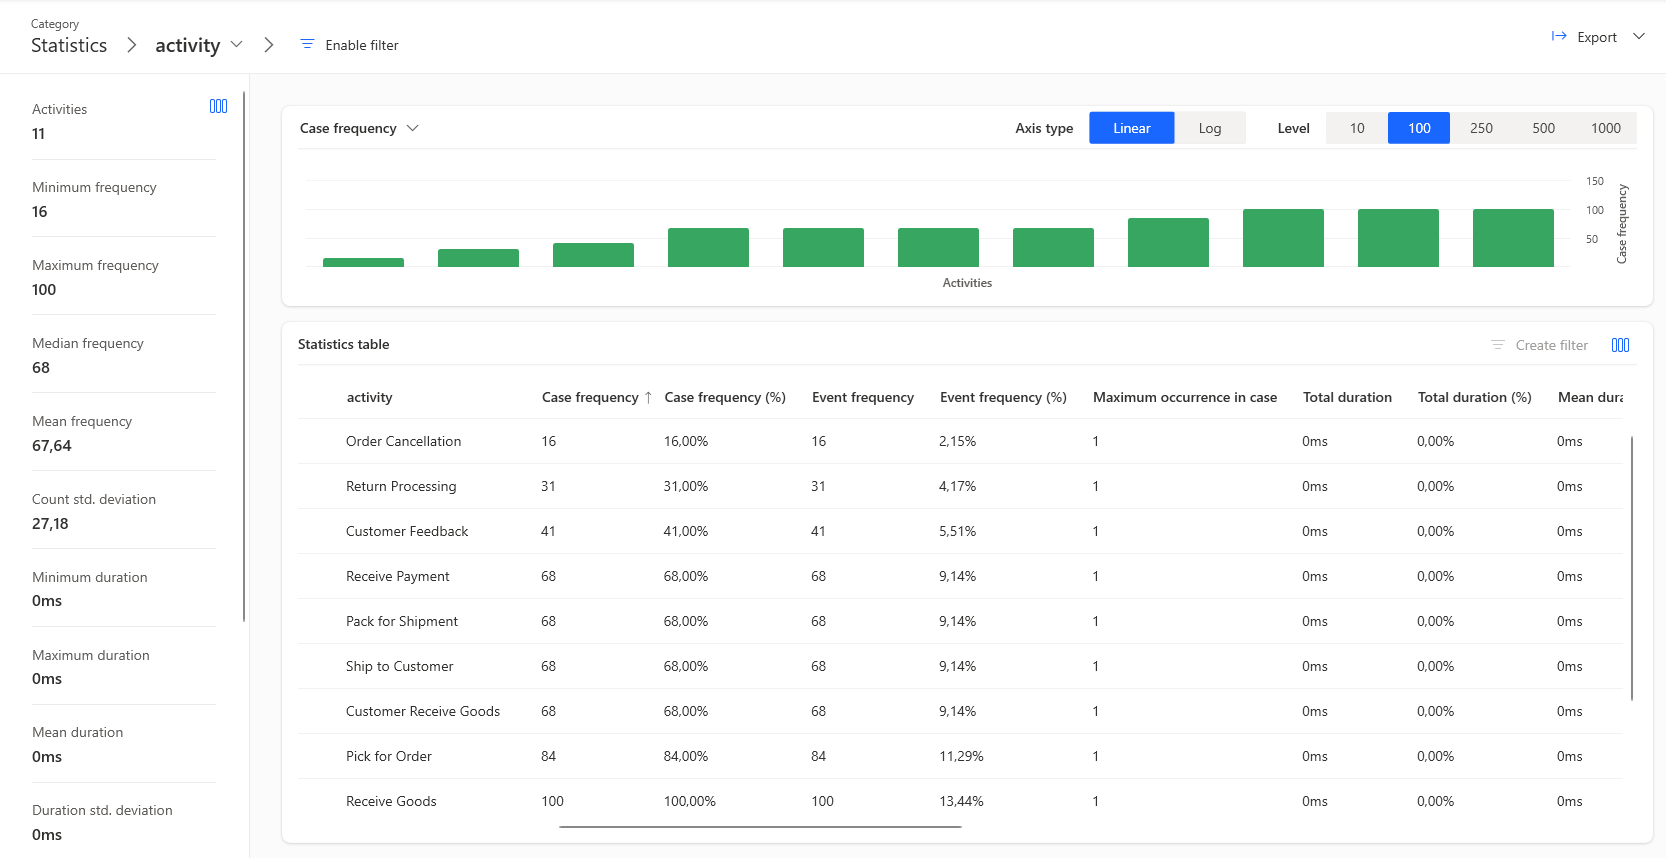
\includegraphics[width=\textwidth]{imgMicrosoft/PrimaSimulazione/StatisticsActivitySimulazione1.png}
    \caption{Statistiche delle attività}
    \label{fig:statistics-activity}
\end{figure}
La schermata delle statistiche sulle attività analizza la frequenza e la distribuzione delle varie fasi operative all'interno del processo aziendale. Le statistiche presentate forniscono una visione dettagliata delle attività svolte, evidenziando la loro frequenza e il loro impatto all'interno del processo.\\
Il pannello delle statistiche mostra che nel processo sono state identificate 11 diverse attività, con una frequenza minima di 16 e una massima di 100 occorrenze. La frequenza mediana è di 68, mentre la media delle frequenze delle attività è di 67,64 con una deviazione standard di 27,18. Questi valori indicano una distribuzione relativamente ampia delle frequenze delle attività, con alcune fasi del processo che si verificano più frequentemente rispetto ad altre.\\
L'attività "Receive Goods" è quella con la frequenza più alta, essendo presente in tutti i casi considerati (100\%). Questo conferma il fatto che la ricezione della merce è un passaggio iniziale essenziale e ricorrente in ogni ciclo operativo.\\
Dall'altra parte, "Order Cancellation" ha la frequenza più bassa, verificandosi solo nel 16\% dei casi. Questo dato è coerente con l'idea che le cancellazioni degli ordini rappresentano un'eccezione nel processo, un'interruzione che si verifica meno frequentemente.\\
La frequenza degli eventi conferma che "Receive Goods" ha la percentuale più alta di occorrenze con il 13,44\% degli eventi totali. Le attività come "Pick for Order," "Receive Payment," "Pack for Shipment," "Ship to Customer," e "Customer Receive Goods" hanno tutte la stessa frequenza di evento del 9,14\%, indicando che queste fasi sono interconnesse e hanno un peso simile nel processo operativo.\\
Le attività di "Return Processing" e "Customer Feedback" si verificano rispettivamente nel 31\% e nel 41\% dei casi, con frequenze di evento inferiori rispetto alle fasi centrali del processo, il che suggerisce che non tutti i clienti forniscono feedback o avviano un reso dopo la ricezione del prodotto.\\
L'analisi delle statistiche sulle attività offre una visione dettagliata della frequenza con cui ciascuna fase del processo viene eseguita. Le fasi iniziali, come la ricezione della merce, sono comuni a tutti i cicli, mentre altre attività, come la cancellazione degli ordini o la gestione dei resi, si verificano meno frequentemente. La distribuzione delle frequenze degli eventi evidenzia che le attività principali del processo sono ben bilanciate, suggerendo una sequenza operativa coerente e standardizzata. Tuttavia, la mancanza di dati sulla durata effettiva delle attività limita l'analisi temporale del processo.

\subsubsection{Edge statistics}
\begin{figure}[H]
    \centering
    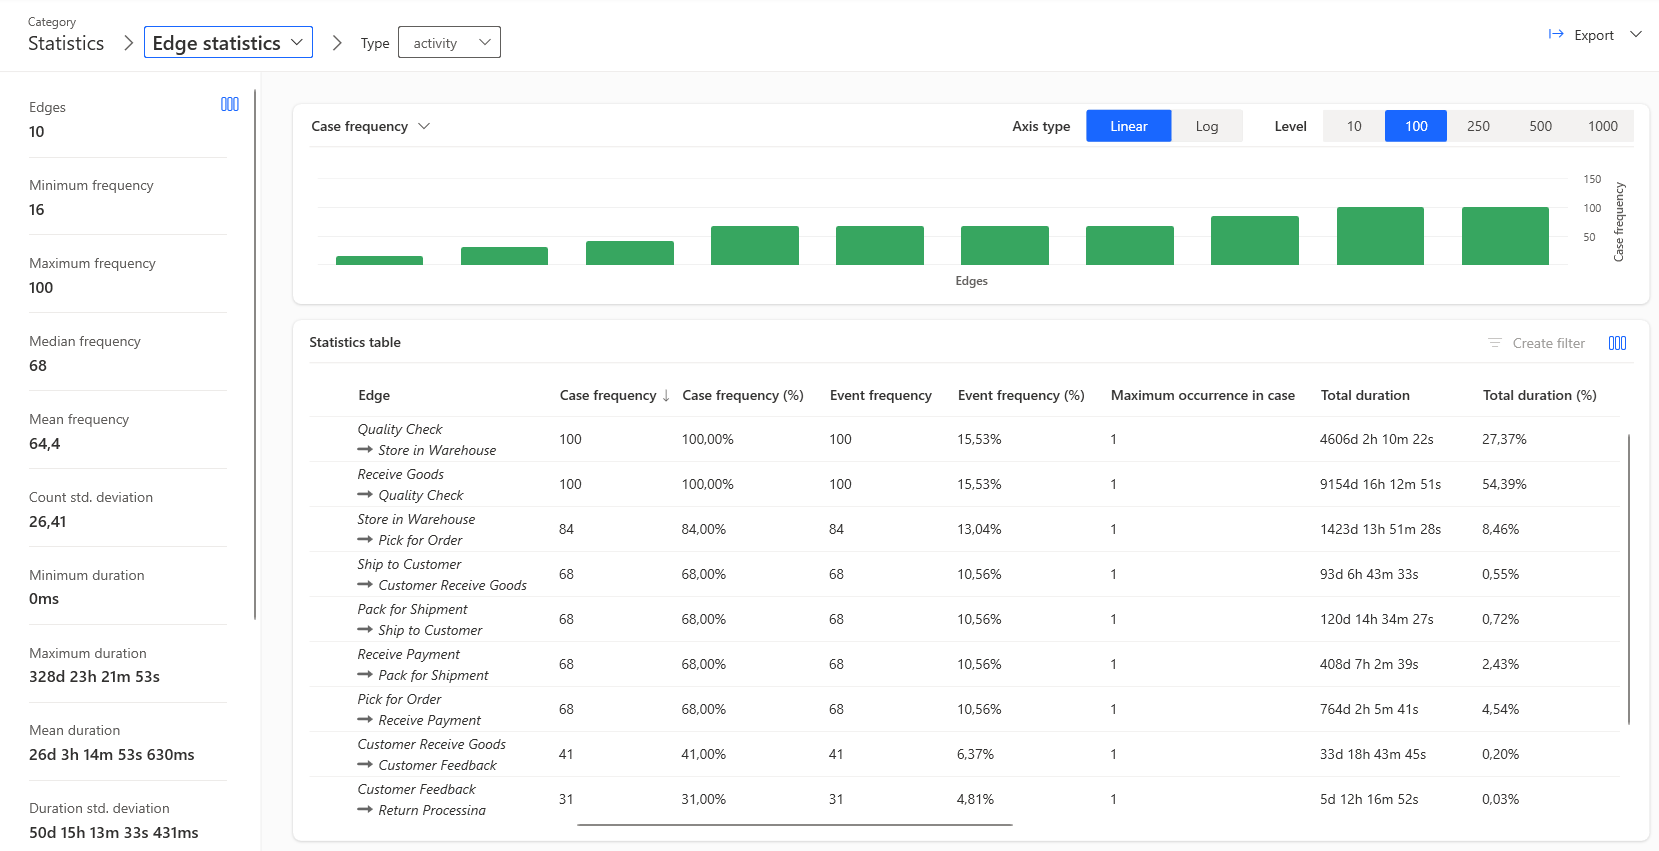
\includegraphics[width=\textwidth]{imgMicrosoft/PrimaSimulazione/StatisticsEdgeStatisticsSimulazione1.png}
    \caption{Statistiche dei collegamenti}
    \label{fig:edge-statistics}
\end{figure}
La schermata delle statistiche dei collegamenti analizza le transizioni tra le attività nel processo aziendale, identificando la frequenza e la durata complessiva di ciascun collegamento. Questi collegamenti rappresentano i passaggi da un'attività all'altra all'interno del flusso di lavoro. L'obiettivo di questa analisi è comprendere meglio come le attività si collegano tra loro, identificare eventuali colli di bottiglia e valutare l'efficienza delle transizioni.\\
La schermata evidenzia che nel processo sono stati identificati 10 collegamenti ("edges") principali, ognuno dei quali rappresenta una transizione tra due attività. La frequenza minima di un collegamento è 16, mentre la massima è 100, con una frequenza mediana di 68 e una media di 64,4. La deviazione standard di 26,41 suggerisce una certa variabilità nella frequenza con cui si verificano queste transizioni.\\
I collegamenti più frequenti sono quelli tra "Receive Goods" e "Quality Check" e tra "Quality Check" e "Store in Warehouse", entrambi con una frequenza del 100\% dei casi. Questo indica che queste transizioni sono fondamentali e avvengono in ogni ciclo del processo, rappresentando le prime fasi essenziali della gestione del prodotto.\\
D'altra parte, collegamenti come "Customer Feedback" verso "Return Processing" sono molto meno frequenti, verificandosi solo nel 31\% dei casi. Questo riflette il fatto che non tutti i clienti avviano un processo di reso dopo aver fornito un feedback, suggerendo una variabilità nelle preferenze e nei comportamenti dei clienti.\\
La durata delle transizioni è un aspetto cruciale per comprendere l'efficienza del processo. Il collegamento "Receive Goods" verso "Quality Check" ha la durata complessiva più lunga, con 9154 giorni, 16 ore e 12 minuti, rappresentando il 54,39\% della durata totale del processo. Questo suggerisce che, nonostante la frequenza elevata, questa fase può essere un collo di bottiglia significativo, potenzialmente rallentando l'intero flusso di lavoro.\\
Al contrario, il collegamento tra "Pack for Shipment" e "Ship to Customer" ha una durata complessiva molto inferiore (120 giorni, 14 ore e 34 minuti), rappresentando solo lo 0,72\% della durata totale del processo. Questo indica che, una volta che il prodotto è pronto per la spedizione, il passaggio verso la consegna è relativamente rapido e fluido.\\
Un altro collegamento di interesse è quello tra "Customer Feedback" e "Return Processing," che ha la durata complessiva più breve (5 giorni, 12 ore e 16 minuti), rappresentando solo lo 0,03\% della durata totale del processo. Questo potrebbe suggerire che il processo di reso, sebbene raro, viene gestito in modo efficiente una volta avviato.\\
La schermata delle statistiche dei collegamenti offre una visione dettagliata delle transizioni tra le attività e della loro influenza sulla durata complessiva del processo. I collegamenti più frequenti si verificano all'inizio del ciclo, segnalando le fasi critiche della gestione del prodotto. Tuttavia, la durata complessiva di alcuni collegamenti, in particolare tra "Receive Goods" e "Quality Check," suggerisce potenziali aree di inefficienza che potrebbero beneficiare di un'ottimizzazione.\\
Nel complesso, l'analisi dei collegamenti mette in luce l'importanza di monitorare non solo la frequenza delle transizioni, ma anche la loro durata, per identificare colli di bottiglia e migliorare l'efficienza del processo aziendale.

\subsubsection{Statistics activity\_id}
\begin{figure}[H]
    \centering
    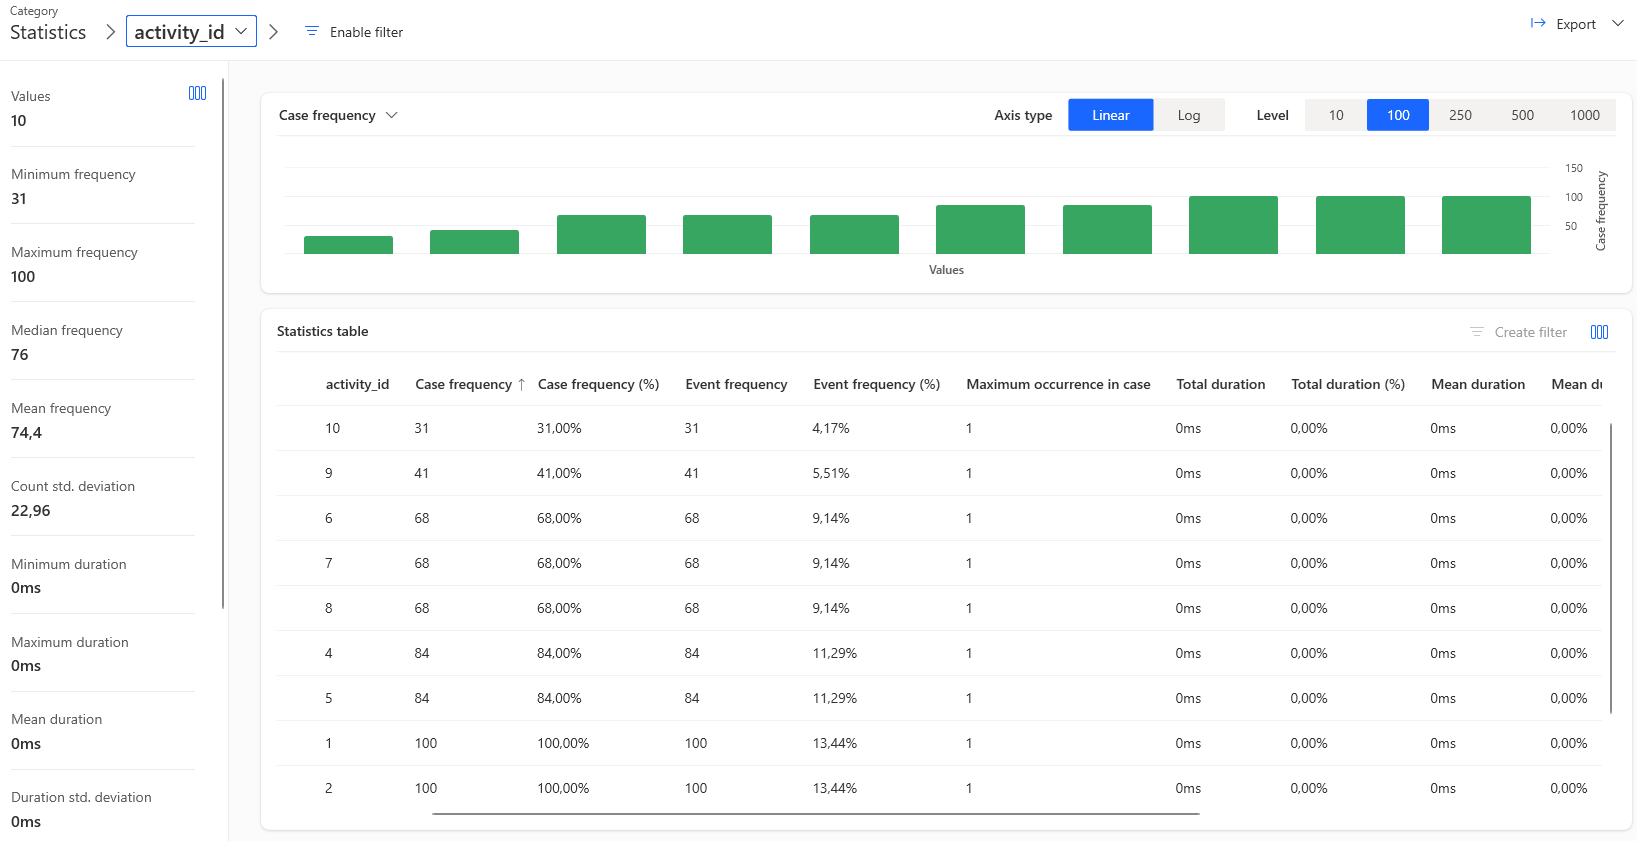
\includegraphics[width=\textwidth]{imgMicrosoft/PrimaSimulazione/StatisticsActivityIdSimulazione1.png}
    \caption{Statistiche degli activity\_id}
    \label{fig:statistics-activity_id}
\end{figure}
La schermata delle statistiche relative agli "Activity ID" fornisce una panoramica dettagliata delle frequenze con cui ciascuna attività identificata si verifica all'interno del processo. Questa analisi è essenziale per comprendere la distribuzione delle attività e il loro peso complessivo nel flusso di lavoro aziendale.\\
La schermata evidenzia che sono stati analizzati 10 diversi Activity ID, con una frequenza minima di 31 e una massima di 100. La frequenza mediana è di 76, mentre la frequenza media delle attività è di 74,4 con una deviazione standard di 22,96. Questi valori indicano una distribuzione abbastanza ampia delle attività, con alcune che si verificano molto più frequentemente rispetto ad altre.\\
Gli Activity ID con la frequenza più alta (100 casi, ovvero il 100\% dei casi) sono quelli associati alle prime fasi del processo. Questo suggerisce che queste attività sono comuni e cruciali, ripetendosi in ogni ciclo operativo del processo.\\
Al contrario, l'Activity ID con la frequenza più bassa (31 casi, pari al 31\% dei casi) rappresenta un'attività che è meno comune e potrebbe essere associata a una parte opzionale o di eccezione del processo, come ad esempio una fase di feedback o di gestione dei resi.\\
L'Event Frequency conferma ulteriormente l'importanza delle attività associate agli Activity ID 1 e 2, che coprono il 13,44\% ciascuno degli eventi totali nel processo. La frequenza degli eventi per gli Activity ID 4 e 5 è inferiore, ma comunque significativa (11,29\% ciascuno), suggerendo che queste attività, sebbene non iniziali, sono comunque centrali nel flusso di lavoro.\\
La schermata delle statistiche degli Activity ID offre una visione chiara e dettagliata della frequenza con cui le diverse attività si verificano nel processo. Le attività con ID 1 e 2, essendo le più frequenti, costituiscono i pilastri del processo, mentre altre attività meno frequenti potrebbero rappresentare fasi opzionali o eccezionali.\\
L'assenza di dati sulle durate delle attività limita l'analisi temporale, ma la distribuzione delle frequenze fornisce comunque preziosi spunti sull'importanza relativa delle diverse fasi del processo. Questi risultati possono essere utilizzati per identificare potenziali aree di miglioramento, ottimizzando le attività meno frequenti o riducendo la necessità di fasi eccezionali.

\subsubsection{Variants}
\begin{figure}[H]
    \centering
    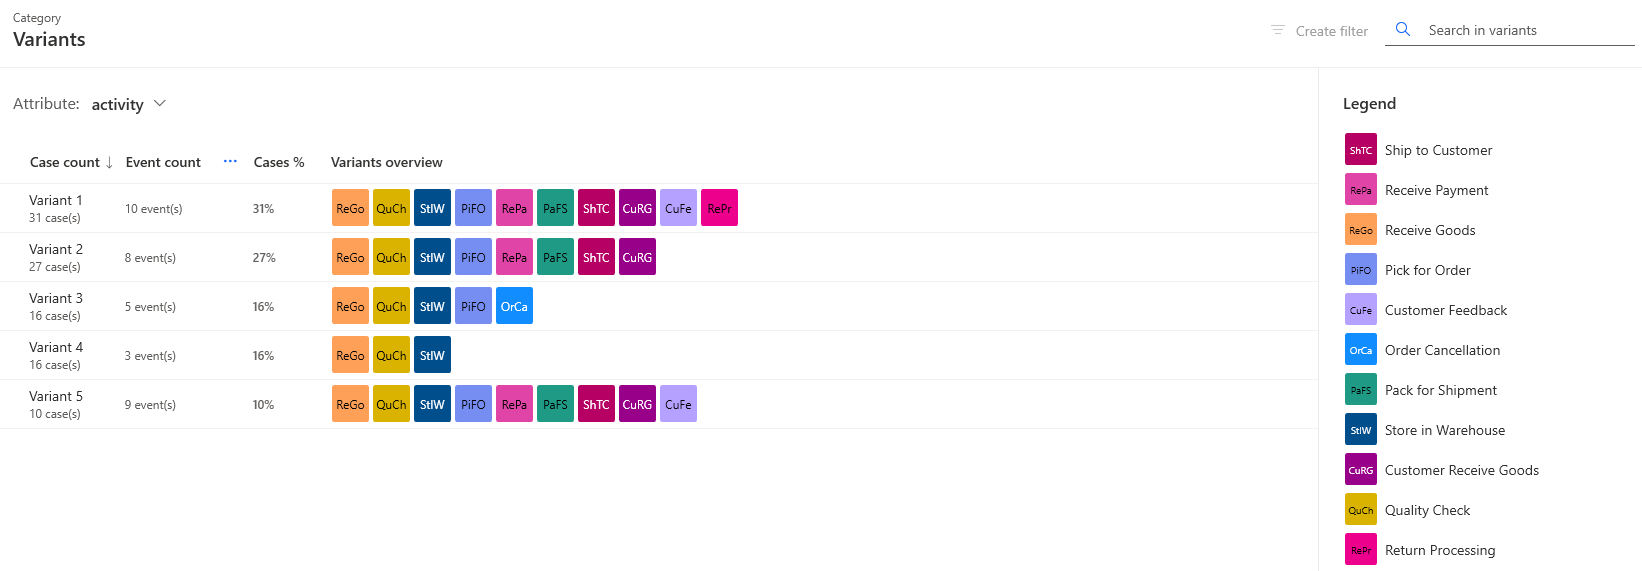
\includegraphics[width=\textwidth]{imgMicrosoft/PrimaSimulazione/VariantsSimulazione1.png}
    \caption{Varianti}
    \label{fig:variants}
\end{figure}
La schermata delle varianti del processo offre una visione dettagliata delle diverse sequenze di attività che possono verificarsi all'interno del flusso di lavoro aziendale. Ogni variante rappresenta un percorso alternativo che un caso può seguire, riflettendo la flessibilità e le possibili deviazioni nel processo. Questa analisi aiuta a comprendere la distribuzione delle varianti e la frequenza con cui ciascuna si verifica.\\
Nella schermata sono identificate cinque varianti principali, ciascuna con una differente sequenza di attività e frequenza di occorrenza:
\begin{itemize}
    \item \custombold{variante 1}: è la più comune, presente in 31 casi, rappresentando il 31\% del totale. Questa variante include 10 attività e segue un percorso completo, dalla ricezione dei beni ("Receive Goods") fino al trattamento dei resi ("Return Processing"). La presenza di tutte queste attività indica che questa variante rappresenta un processo completo e robusto, che include fasi opzionali come il feedback del cliente e la gestione dei resi;
    \item \custombold{variante 2}: copre il 27\% dei casi, è leggermente più corta, con 8 attività. In questa variante, il processo termina dopo la ricezione del prodotto da parte del cliente, senza coinvolgere il feedback o il trattamento dei resi. Questo potrebbe indicare un flusso di lavoro in cui i clienti non forniscono feedback o in cui i resi non sono richiesti;
    \item \custombold{variante 3}: rappresenta il 16\% dei casi ed è ancora più breve, con solo 5 attività. Questa variante include la cancellazione dell'ordine ("Order Cancellation") dopo il prelievo del prodotto, indicando che il processo si interrompe prematuramente per una parte significativa dei casi;
    \item \custombold{variante 4}: in questa variante, il processo si ferma dopo la conservazione in magazzino, suggerendo che una parte dei prodotti potrebbe non essere mai ordinata o preparata per la spedizione;
    \item \custombold{variante 5}: questa variante include 9 attività e termina con il feedback del cliente, senza però passare attraverso il trattamento dei resi. Questo flusso di lavoro rappresenta i casi in cui i clienti forniscono un feedback ma non effettuano resi, il che può indicare un alto livello di soddisfazione del cliente.
\end{itemize}
L'analisi delle varianti evidenzia la flessibilità e la complessità del processo aziendale. Le varianti più lunghe, come la Variante 1, rappresentano percorsi completi che includono tutte le possibili fasi del processo, mentre le varianti più corte indicano flussi di lavoro semplificati o interrotti.\\
La distribuzione delle varianti suggerisce che la maggior parte dei casi segue un percorso completo o quasi completo, con solo una minoranza che si ferma prematuramente. Questa comprensione delle varianti può aiutare a ottimizzare il processo, identificando quali fasi possono essere eliminate o migliorate per aumentare l'efficienza e la soddisfazione del cliente.

\subsection{Seconda simulazione}
Il file CSV è stato creato mediante uno script Python che simula una serie di attività relative alla produzione e alla gestione degli ordini di prodotti. Inoltre, per la simulazione dei dati, sono stati presi in considerazione anche i dati estratti manualmente da un database di un sistema gestionale.
\subsubsection{Regole di simulazione dei dati}
\custombold{Impostazione delle date iniziali}\\
Ogni ciclo di attività inizia con la prima attività programmata tra il 1 gennaio 2019 e il 31 dicembre 2020.\\
\custombold{Definizione delle tipologie di prodotti}\\
Viene creata una lista di 30 tipi di scarpe, denominate "Scarpe tipo 1" fino a "Scarpe tipo 30".\\
\custombold{Definizione delle attività e delle durate}\\
Sono state definite 17 attività, ciascuna con un ID unico e una durata variabile. Le durate delle attività sono espresse in minuti o giorni, a seconda dell'attività specifica.\\
\custombold{Generazione di un ciclo di attività per prodotto}\\
Per ciascun prodotto, viene generato un ciclo di attività che segue le seguenti regole:
\begin{itemize}
    \item \custombold{attività obbligatorie}: alcune attività avvengono in un ordine fisso. Ad esempio, "COnferma ordine" è sempre seguita da "Creazione progetto";
    \item \custombold{modifica del progetto}: un numero casuale di modifiche al progetto (da 1 a 5) può essere aggiunto dopo la creazione del progetto;
    \item \custombold{gestione degli ordini fornitore}: un numero casuale (da 1 a 3) di cicli di gestione ordini fornitore può essere inserito, ognuno dei quali può includere attività come "Ordine fornitore", "Arrivo offerta fornitore", "Ordine annullato", o "Ordine sospeso";
    \item \custombold{produzione}: vengono aggiunte attività relative alla produzione, come "Stampa scheda di produzione", "Inizio ciclo di produzione" e "Termine ordine di produzione";
    \item \custombold{fatturazione e consegna}: dopo la produzione, vengono aggiunte le attività di "Invio fattura cliente" e "Consegna". La ricezione del pagamento della fattura può avvenire in modo casuale prima o dopo la consegna, ma deve avvenire almeno una volta per ciclo.
\end{itemize}
\custombold{Generazione dei timestamp}\\
Ogni attività riceve un timestamp generato casualmente basato su un intervallo di tempo definito per quella specifica attività.\\
\custombold{Ciclo di generazione dei dati}\\
Il numero di prodotti varia tra 300 e 500, determinato casualmente. Per ogni prodotto, viene generato un ciclo di attività completo, assicurandosi che tutte le attività obbligatorie siano inserite nel corretto ordine e che le attività casuali siano distribuite come specificato.

\subsubsection{Process map}
\begin{figure}[H]
    \centering
    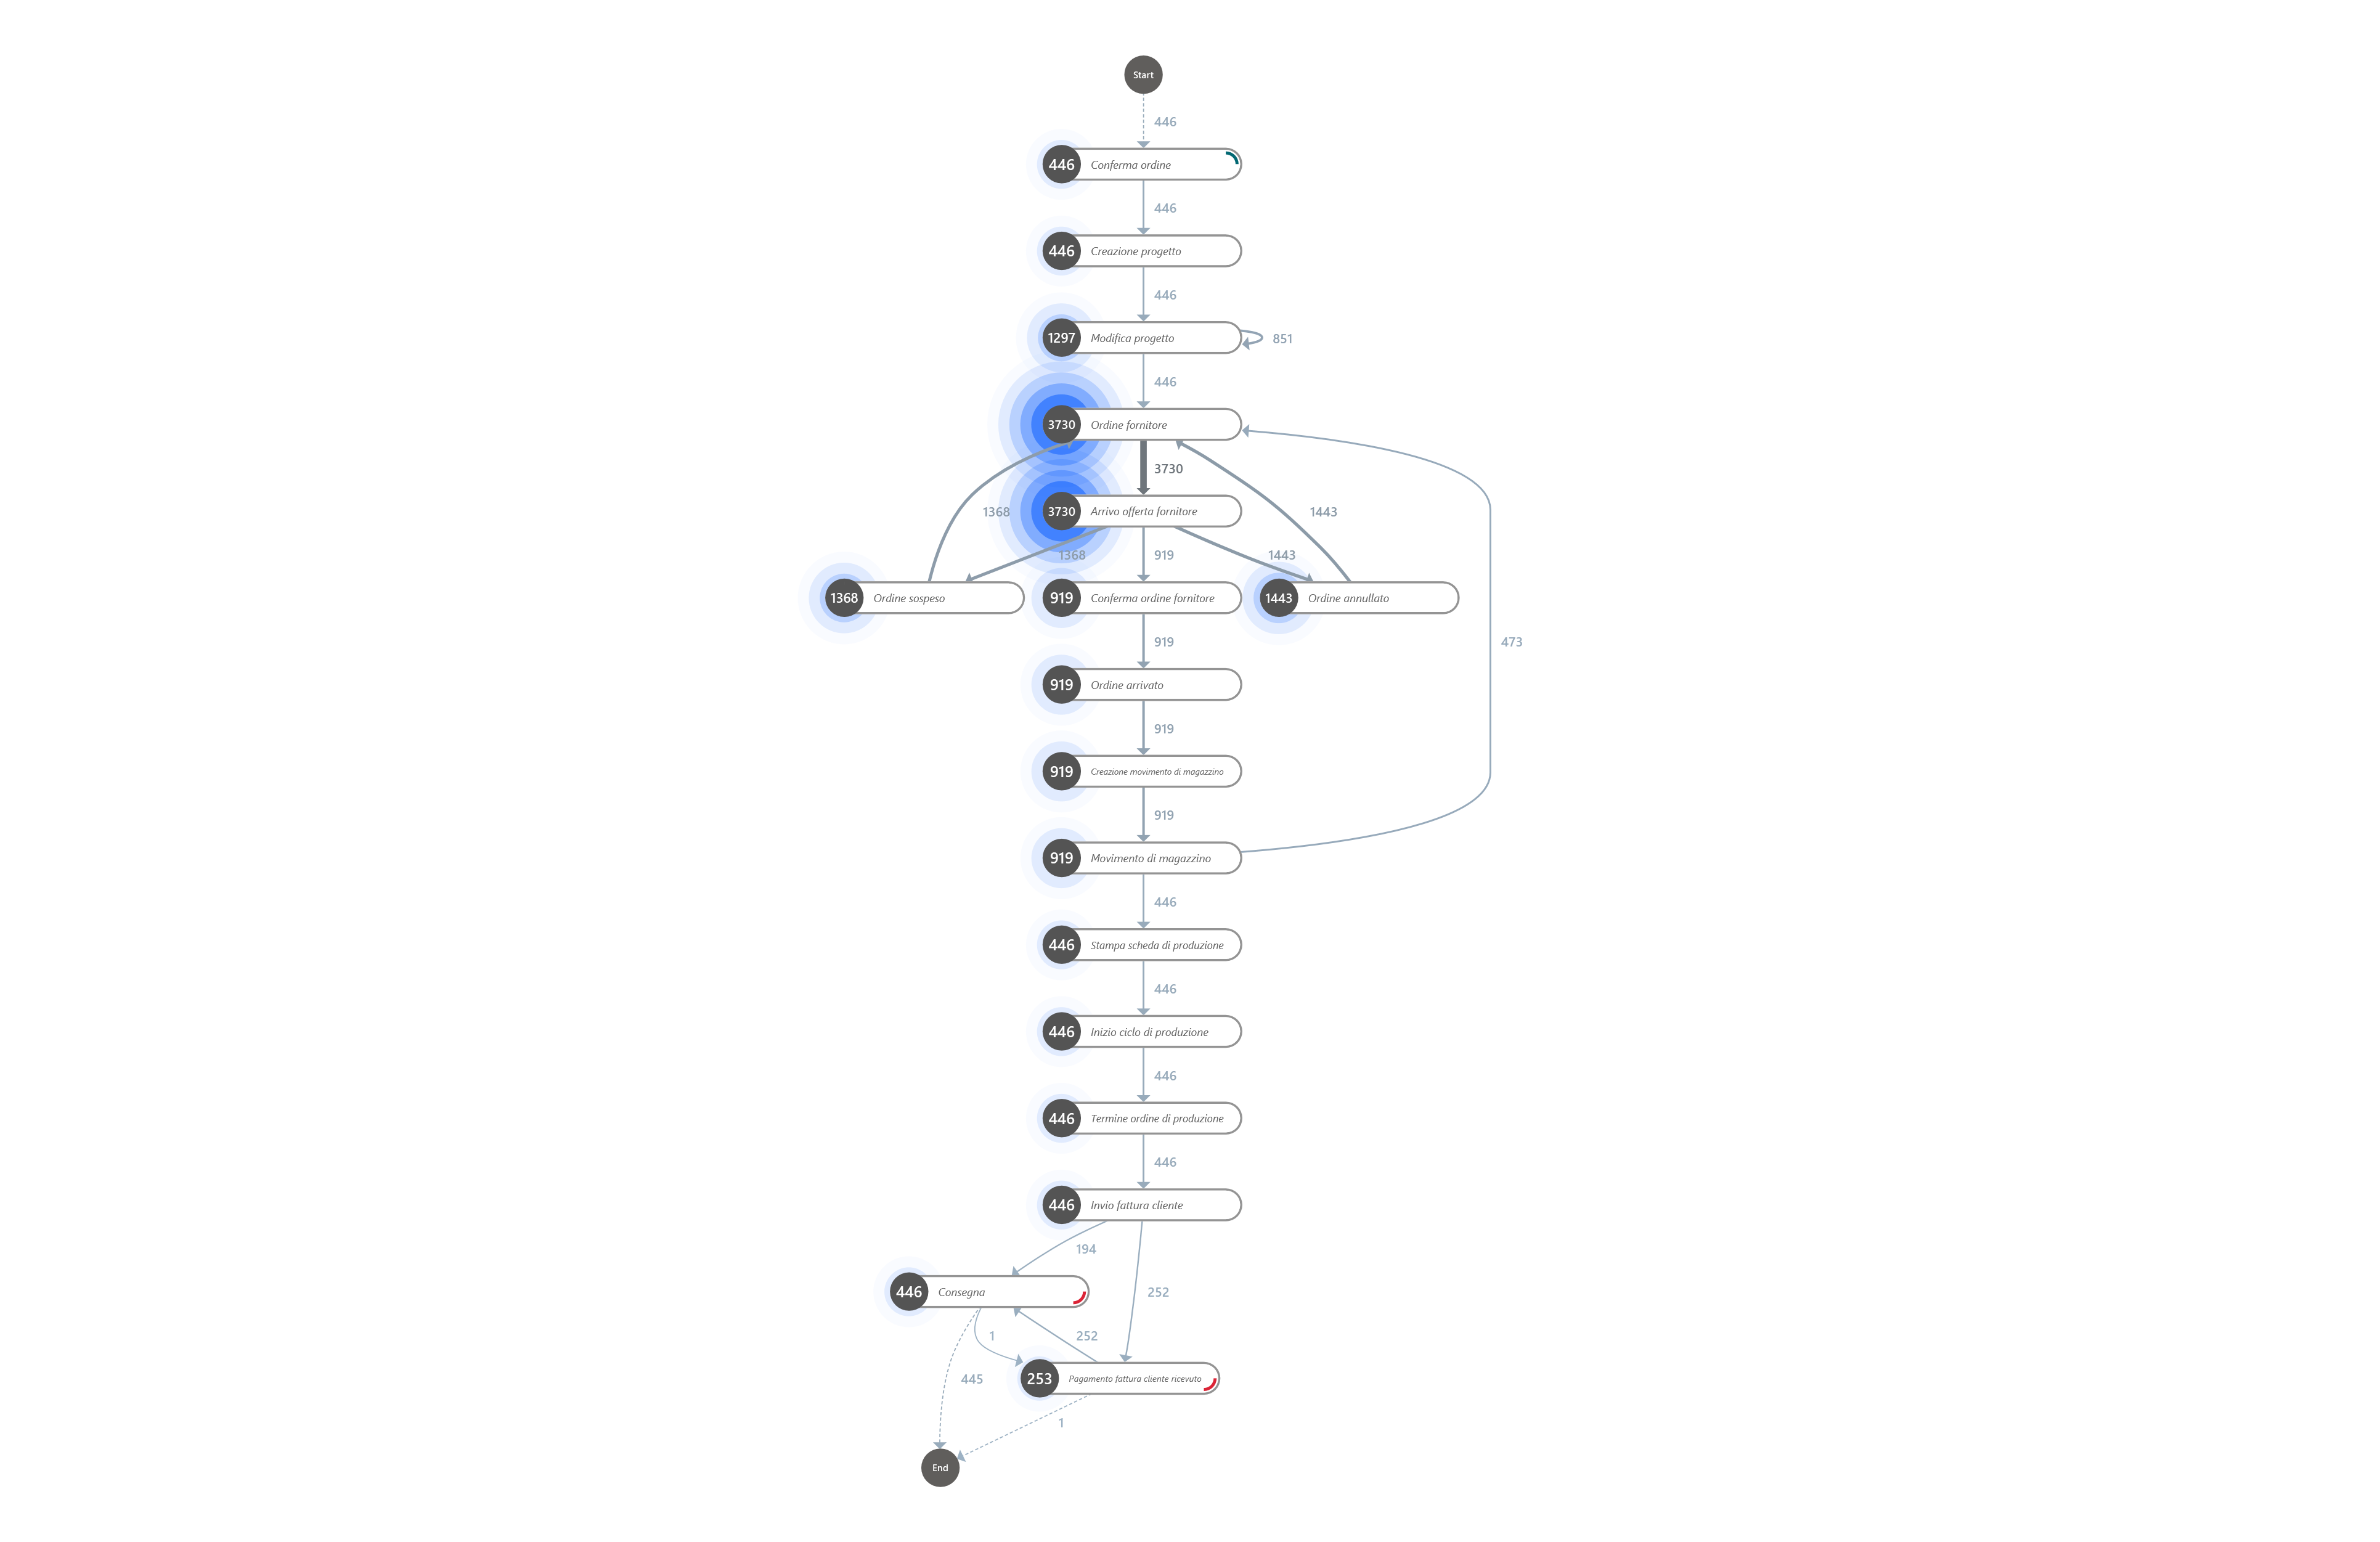
\includegraphics[width=\textwidth]{imgMicrosoft/SecondaSimulazione/ProcessMapSimulazione2.png}
    \caption{Mappa del processo}
    \label{fig:process-map}
\end{figure}
Il processo inizia con la conferma dell'ordine ("Conferma ordine"), seguita dalla creazione del progetto ("Creazione progetto"). Questo è un percorso obbligato per ogni ciclo, come previsto dalle regole di simulazione dei dati. In alcuni casi, segue la modifica del progetto ("Modifica progetto"), che può essere ripetuta più volte, evidenziando la possibilità di revisioni multiple prima di procedere con l'ordine al fornitore.\\
Il processo continua con la gestione degli ordini al fornitore, dove possono verificarsi diverse varianti come l'arrivo dell'offerta ("Arrivo offerta fornitore"), l'annullamento dell'ordine ("Ordine annullato"), o la sospensione dell'ordine ("Ordine sospeso"). Queste varianti sono chiaramente rappresentate nella mappa, mostrando la flessibilità del processo e le decisioni che possono portare a percorsi alternativi.\\
Dopo la conferma dell'ordine da parte del fornitore, il processo procede verso la fase di produzione, che include attività come la stampa della scheda di produzione ("Stampa scheda di produzione"), l'inizio del ciclo di produzione ("Inizio ciclo di produzione"), e il termine dell'ordine di produzione ("Termine ordine di produzione"). Queste fasi sono rappresentate in sequenza, mostrando un flusso lineare e ben definito.\\
Infine, il processo si conclude con l'invio della fattura al cliente ("Invio fattura cliente") e la consegna del prodotto ("Consegna"). È interessante notare che il pagamento della fattura ("Pagamento fattura cliente") può avvenire in modo casuale prima o dopo la consegna, come previsto dalle regole di simulazione. La mappa mostra chiaramente questo aspetto, evidenziando i percorsi alternativi che portano alla conclusione del ciclo.\\
La mappa di processo mostra una struttura ben organizzata, con percorsi chiari e collegamenti logici tra le attività. Le dimensioni delle bolle e le connessioni tra di esse riflettono la frequenza e l'importanza delle transizioni, permettendo di identificare facilmente le attività principali e i punti di decisione critici.
Un aspetto notevole è la presenza di percorsi alternativi e cicli, in particolare nella fase di gestione degli ordini al fornitore, che indicano la complessità e la flessibilità del processo. Questo è coerente con la simulazione, che prevede la possibilità di modifiche al progetto e cicli di gestione degli ordini che possono variare in base alle circostanze.\\
Inoltre, la mappa evidenzia anche le attività che rappresentano potenziali colli di bottiglia, come la "Modifica progetto" e la "Consegna", dove potrebbero verificarsi ritardi. Queste informazioni sono cruciali per il monitoraggio del rispetto delle scadenze, una funzionalità chiave nel contesto della simulazione.\\
La mappa di processo fornisce una rappresentazione dettagliata e coerente del flusso di lavoro simulato, evidenziando sia le fasi obbligatorie che le varianti possibili. La struttura della mappa riflette accuratamente le regole di simulazione, offrendo una visione chiara delle diverse possibilità all'interno del ciclo di produzione e gestione degli ordini.

\subsubsection{Statistics case overview}
\begin{figure}[H]
    \centering
    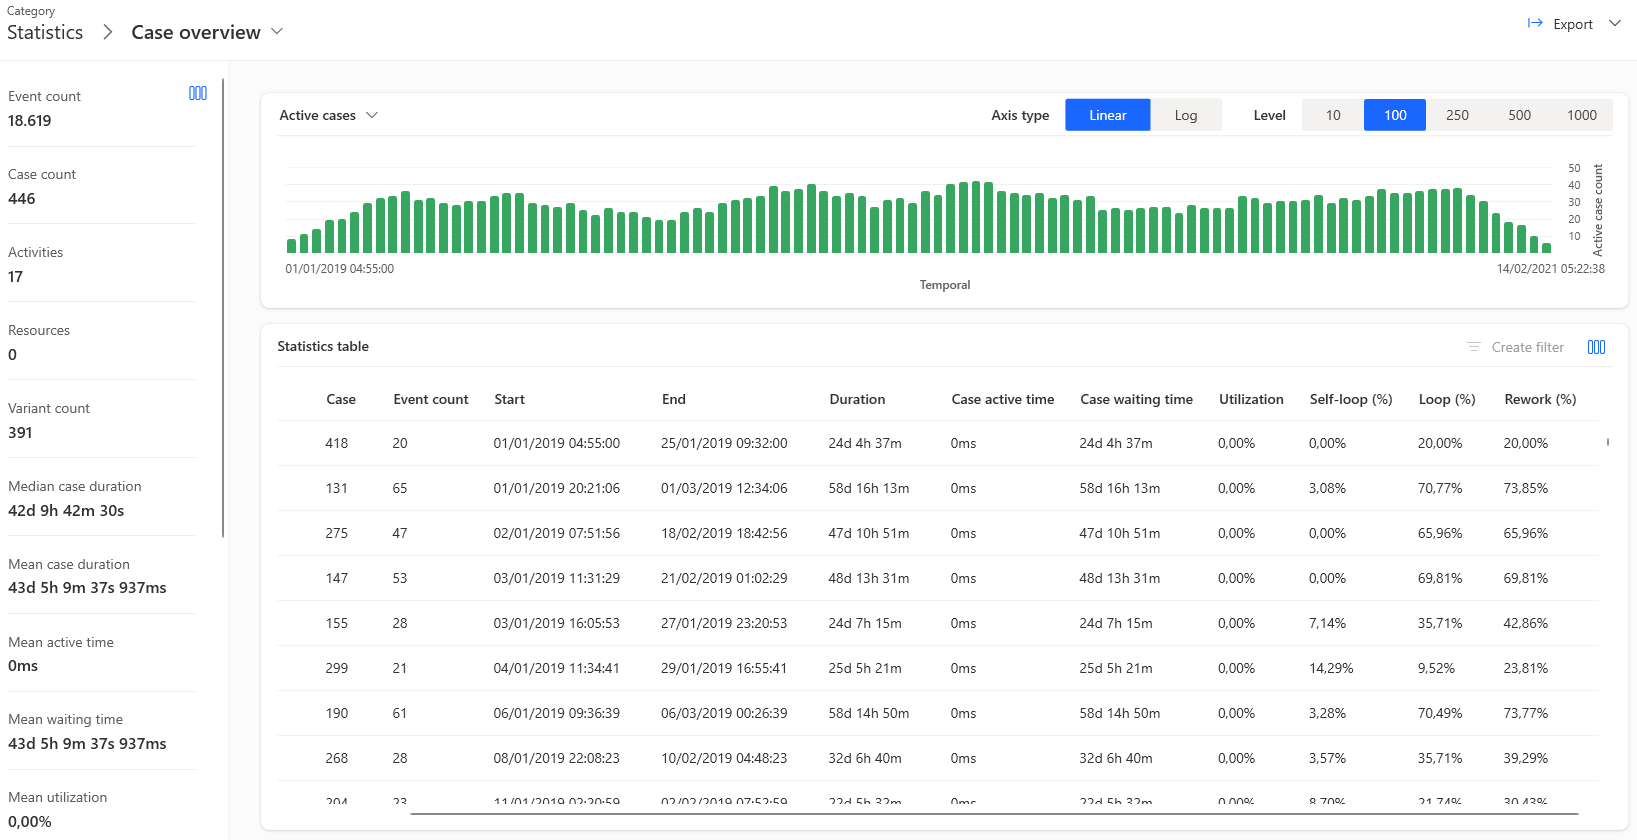
\includegraphics[width=\textwidth]{imgMicrosoft/SecondaSimulazione/StatisticsCaseOverviewSimulazione2.png}
    \caption{Statistiche dei casi}
    \label{fig:statistics-case-overview}
\end{figure}
La schermata di panoramica dei casi fornisce un'analisi dettagliata delle attività di produzione e gestione degli ordini simulati. Questa analisi include il conteggio degli eventi, la durata dei casi, i tempi di attesa, e altri indicatori chiave di performance. Il contesto di questa simulazione è la gestione di un processo produttivo per una serie di prodotti (scarpe) con variazioni nel flusso di lavoro a seconda delle specifiche esigenze e condizioni.\\
La schermata evidenzia che sono stati registrati 18.619 eventi distribuiti su 446 casi. Il numero di attività coinvolte è 17, e sono state identificate 391 varianti del processo, indicando una notevole flessibilità e complessità nella gestione dei casi.\\
La durata mediana di un caso è di 42 giorni, 9 ore, 42 minuti e 30 secondi, con una durata media leggermente superiore di 43 giorni, 5 ore, 9 minuti e 37 secondi. Questa piccola differenza tra mediana e media suggerisce una distribuzione relativamente simmetrica delle durate dei casi, con alcuni casi che possono avere una durata significativamente maggiore o minore rispetto alla media.\\
Il tempo di attesa medio per i casi coincide esattamente con la durata media dei casi (43 giorni, 5 ore, 9 minuti e 37 secondi), indicando che non vi è tempo attivo registrato nei dati. Questo potrebbe essere dovuto alla natura del processo simulato, dove le attività sono distribuite nel tempo senza intervalli di inattività significativa o in cui il tempo di inattività non è stato catturato nei dati.
L'utilizzo medio riportato è 0,00\%, il che suggerisce che le risorse non sono state considerate.\\
Un aspetto interessante emerso dall'analisi è la presenza di cicli o "loop" all'interno dei casi, con alcune varianti che mostrano alti livelli di "self-loop" e rework (ad esempio, il caso 131 con il 70,77\% di loop e 73,85\% di rework). Questi cicli possono indicare revisioni ripetute o attività ripetitive che si verificano all'interno dello stesso caso, come nel caso di modifiche multiple al progetto o ripetizioni di ordini.\\
La presenza di cicli elevati e rework è indicativa della complessità e della possibilità di inefficienze nel processo. La gestione di questi cicli può essere critica per ottimizzare il flusso di lavoro e ridurre i tempi di produzione.\\
Il grafico degli "Active cases" mostra come il numero di casi attivi varia nel tempo, con un picco durante i mesi centrali del periodo considerato. Questo potrebbe riflettere cicli stagionali nella produzione o nella domanda dei prodotti. Verso la fine del periodo, si nota una diminuzione graduale del numero di casi attivi, il che potrebbe indicare un rallentamento delle operazioni o il completamento del ciclo produttivo.\\
La schermata di panoramica dei casi della seconda simulazione offre una visione approfondita della durata e della complessità del processo produttivo. La presenza di numerose varianti e cicli di rework suggerisce un processo altamente flessibile ma potenzialmente inefficiente. La distribuzione temporale dei casi attivi indica un flusso di lavoro variabile con picchi e cali che potrebbero essere correlati a fattori esterni o interni al processo produttivo.\\

\subsubsection{Statistiche per nome attività}
\begin{figure}[H]
    \centering
    \includegraphics[width=\textwidth]{imgMicrosoft/SecondaSimulazione/StatisticsNomeAttivitàSimulazione2.png}
    \caption{Statistiche per nome dell'attività}
    \label{fig:statistics-nome-attività}
\end{figure}
La schermata delle statistiche per "Nome attività" fornisce un'analisi dettagliata della frequenza con cui ciascuna attività si verifica all'interno del processo simulato. La simulazione coinvolge 17 attività diverse, e questa schermata aiuta a comprendere meglio la distribuzione e l'importanza relativa di ogni attività nel flusso di lavoro.\\
Le attività analizzate mostrano una significativa variabilità nella frequenza con cui si verificano. La frequenza minima osservata è di 253 occorrenze, mentre la massima è di 3.730 occorrenze. La frequenza mediana delle attività è di 919, con una media di 1.095,24 e una deviazione standard di 1.026,25. Questi valori indicano che alcune attività sono molto più comuni di altre, suggerendo una centralità maggiore nel processo produttivo.\\
Le attività con la frequenza più alta includono:
\begin{itemize}
    \item "Ordine fornitore" e "Arrivo offerta fornitore" con 3.730 eventi ciascuna, rappresentano una parte essenziale e ripetuta del processo. La loro elevata frequenza riflette il ciclo continuo di gestione degli ordini con i fornitori, una fase cruciale nel processo produttivo;
    \item "Conferma ordine," "Creazione progetto," "Modifica progetto," "Ordine fornitore" e "Arrivo offerta fornitore," tutte con una frequenza del 100\%, sono attività che avvengono in ogni ciclo del processo. Queste attività costituiscono i pilastri del flusso di lavoro, connessi alla fase iniziale e di pianificazione del processo produttivo.
\end{itemize}
D'altra parte, attività come "Pagamento fattura cliente ricevuto" hanno una frequenza più bassa, con il 56,73\% dei casi. Questo potrebbe indicare che non tutte le transazioni vengono completate con la ricezione del pagamento, o che il pagamento può essere registrato in momenti diversi o meno frequentemente rispetto ad altre attività.\\
L'Event Frequency riflette ulteriormente l'importanza delle attività. Per esempio, "Ordine fornitore" e "Arrivo offerta fornitore" coprono ciascuna il 20,03\% degli eventi totali, rendendole le attività più significative in termini di volume. Queste attività non solo si verificano in tutti i casi, ma sono anche ripetute più volte all'interno dello stesso caso, come indicato dal numero massimo di occorrenze in un singolo caso (fino a 20 volte per "Ordine fornitore").\\
La presenza di "Ordine sospeso" e "Ordine annullato" con frequenze del 89,91\% e 90,58\%, rispettivamente, indica che una parte consistente degli ordini può incontrare problemi, necessitando di interventi o modifiche che deviano dal flusso principale.\\
La schermata delle statistiche per "Nome attività" evidenzia la centralità di alcune attività all'interno del processo simulato, in particolare quelle legate alla gestione degli ordini e al rapporto con i fornitori. Le attività come "Conferma ordine" e "Creazione progetto" sono fondamentali e presenti in tutti i cicli, mentre altre, come la ricezione del pagamento, sono meno frequenti e possono indicare variabilità nel completamento del ciclo di produzione.\\
L'analisi suggerisce che il processo è altamente dipendente dalle interazioni con i fornitori, con numerose ripetizioni di ordini e offerte. Le attività meno frequenti, come "Pagamento fattura cliente ricevuto," potrebbero rappresentare opportunità di miglioramento per ottimizzare la conclusione del ciclo e garantire un flusso più fluido.

\subsubsection{Edge statistics}
\begin{figure}[H]
    \centering
    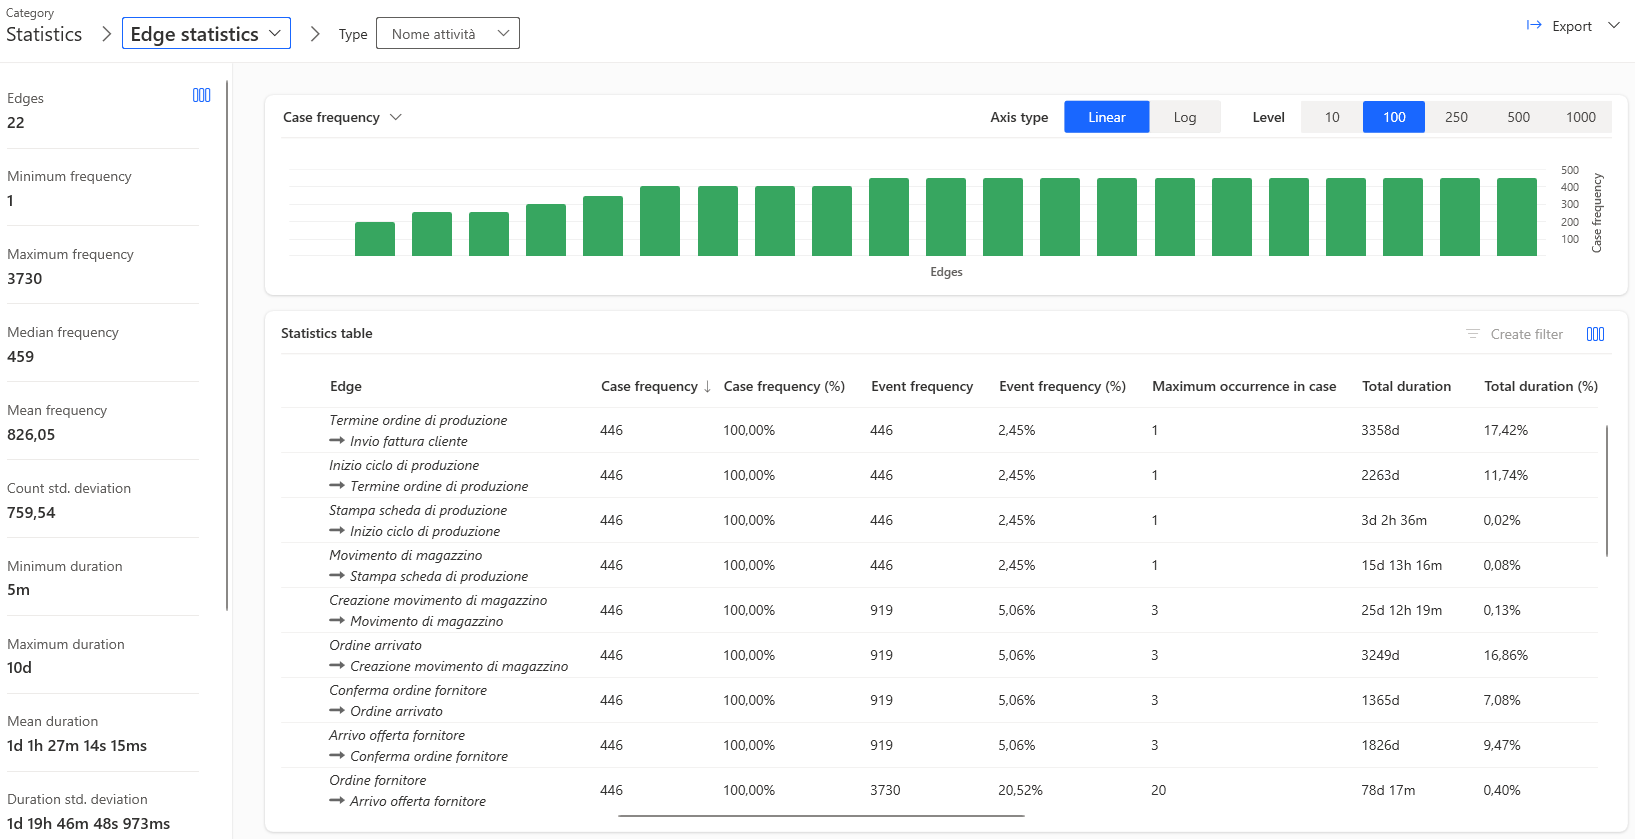
\includegraphics[width=\textwidth]{imgMicrosoft/SecondaSimulazione/StatisticsEdgeStatisticsSimulazione2.png}
    \caption{Statistiche dei collegamenti}
    \label{fig:edge-statistics}
\end{figure}
La schermata delle statistiche dei collegamenti analizza le transizioni tra le diverse attività (o "edges") all'interno del processo produttivo simulato.\\
Nella schermata sono identificati 22 collegamenti principali tra le attività, con una frequenza minima di 1 e una massima di 3.730. La frequenza mediana dei collegamenti è 459, mentre la media è 826,05 con una deviazione standard di 759,54. Questi valori indicano una distribuzione abbastanza ampia delle frequenze, suggerendo che alcune transizioni sono molto più comuni di altre all'interno del processo.\\
I collegamenti più frequenti sono:
\begin{itemize}
    \item "Ordine fornitore" $\rightarrow$ "Arrivo offerta fornitore" con 3.730 occorrenze, rappresenta il 20,52\% della frequenza totale degli eventi. Questo collegamento è cruciale e riflette la natura ripetitiva della gestione degli ordini, che è una parte fondamentale del processo;
    \item "Movimento di magazzino" $\rightarrow$ "Stampa scheda di produzione" e "Creazione movimento di magazzino" $\rightarrow$ "Movimento di magazzino," entrambi con 919 occorrenze ciascuno, rappresentano il 5,06\% della frequenza totale degli eventi. Questi collegamenti indicano la transizione tra la preparazione dei materiali e l'inizio della produzione, una fase chiave nella catena di produzione.
\end{itemize}
Ogni collegamento è accompagnato da una "Case frequency" del 100\%, suggerendo che questi percorsi sono seguiti in tutti i casi simulati, il che conferma la loro importanza all'interno del flusso di lavoro.\\
La durata complessiva di alcune transizioni è significativa, con alcune che rappresentano una parte importante della durata totale del processo:
\begin{itemize}
    \item "Termine ordine di produzione" $\rightarrow$ "Invio fattura cliente" ha una durata totale di 3.358 giorni, rappresentando il 17,42\% della durata complessiva del processo. Questo potrebbe indicare un ritardo o una fase di attesa significativa tra la conclusione della produzione e l'emissione della fattura;
    \item "Ordine arrivato" $\rightarrow$ "Creazione movimento di magazzino," con una durata di 3.249 giorni (16,86\% della durata totale), indica un altro possibile collo di bottiglia dove il processo potrebbe rallentare prima che i materiali vengano registrati e trasferiti al magazzino.
\end{itemize}
Altre transizioni, come "Stampa scheda di produzione" $\rightarrow$ "Inizio ciclo di produzione," hanno durate molto più brevi, suggerendo che una volta avviata, la produzione prosegue in modo relativamente rapido e senza significativi ritardi.\\
La schermata delle statistiche dei collegamenti evidenzia l'importanza di alcune transizioni chiave nel processo produttivo simulato. Le transizioni tra "Ordine fornitore" e "Arrivo offerta fornitore" sono le più frequenti, indicando un focus significativo sulla gestione degli ordini. Tuttavia, la durata estesa di alcuni collegamenti, come quelli tra la conclusione della produzione e l'invio della fattura, suggerisce aree di potenziale inefficienza che potrebbero essere ottimizzate.

\subsubsection{Statistiche prodotto}
\begin{figure}[H]
    \centering
    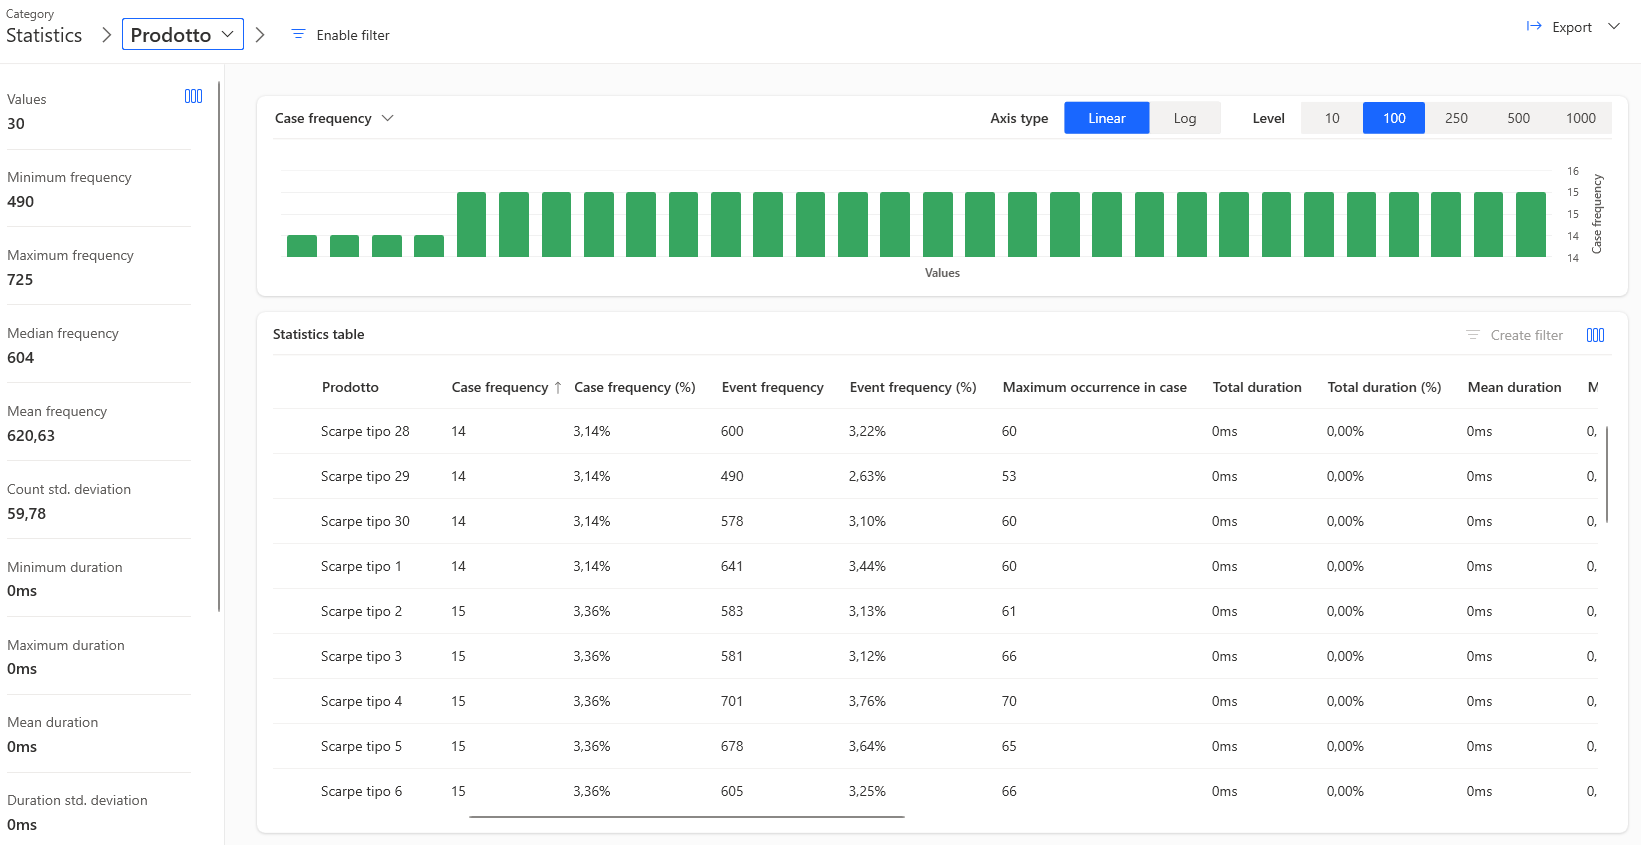
\includegraphics[width=\textwidth]{imgMicrosoft/SecondaSimulazione/StatisticsProdottoSimulazione2.png}
    \caption{Statistiche dei prodotti}
    \label{fig:statistics-prodotto}
\end{figure}
La schermata delle statistiche per "Prodotto" analizza la frequenza e la distribuzione delle attività relative ai 30 diversi tipi di scarpe simulate nel processo. Ogni prodotto è rappresentato da un caso specifico, e questa schermata fornisce un quadro chiaro di come ogni tipo di scarpa sia gestito all'interno del flusso di lavoro.\\
La schermata evidenzia che le frequenze dei casi per i vari prodotti sono relativamente omogenee, con un minimo di 490 occorrenze e un massimo di 725. La frequenza mediana è 604, mentre la media è 620,63 con una deviazione standard di 59,78. Questo indica una distribuzione abbastanza equilibrata tra i diversi tipi di scarpe, suggerendo che tutti i prodotti sono trattati in modo simile all'interno del processo.\\
I prodotti con la frequenza più alta sono gestiti con un numero maggiore di eventi, suggerendo che potrebbero essere soggetti a cicli di lavorazione più complessi o a un maggiore numero di attività. Ad esempio:
\begin{itemize}
    \item \custombold{scarpe tipo 3}: ha una frequenza di 15 casi con 701 eventi, il che rappresenta un 3,76\% della frequenza totale degli eventi. Questo potrebbe indicare una maggiore complessità o un numero maggiore di passaggi nel processo per questo tipo di scarpa;
    \item \custombold{scarpe tipo 1}: con 641 eventi, rappresenta un 3,44\% della frequenza totale degli eventi, che è anch'essa significativa e può riflettere un ciclo operativo robusto.
\end{itemize}
D'altra parte, prodotti come \custombold{scarpe tipo 29} hanno una frequenza di 14 casi con 490 eventi, che è leggermente inferiore rispetto ad altri prodotti, suggerendo che potrebbero essere gestiti con un processo leggermente meno complesso o con meno attività ripetitive.\\
La frequenza degli eventi per ciascun prodotto varia, ma rimane generalmente bilanciata. Questo equilibrio tra i diversi prodotti indica che il processo produttivo è stato progettato per trattare i vari tipi di scarpe con un livello simile di attenzione e complessità:
\begin{itemize}
    \item \custombold{scarpe tipo 4}: presenta il massimo numero di eventi (701) tra tutti i prodotti analizzati, il che potrebbe indicare che questo prodotto richiede un processo più lungo o più iterazioni di attività rispetto agli altri;
    \item \custombold{scarpe tipo 29}: con il numero minimo di eventi (490), potrebbe rappresentare un prodotto con un processo più semplice o con meno iterazioni richieste.
\end{itemize}
La schermata delle statistiche per prodotto mostra che c'è una distribuzione abbastanza uniforme delle attività tra i diversi tipi di scarpe. Alcuni prodotti, come le Scarpe tipo 3 e tipo 4, richiedono un maggior numero di eventi, suggerendo una maggiore complessità nel loro ciclo produttivo. Tuttavia, la deviazione standard relativamente bassa indica che il processo è ben bilanciato tra i vari prodotti.\\
Questa uniformità suggerisce che il sistema di produzione è progettato per trattare tutti i tipi di scarpe in modo simile, garantendo che nessun prodotto sia trascurato o gestito in modo inefficiente.

\subsubsection{Root cause analysis}
\begin{figure}[H]
    \centering
    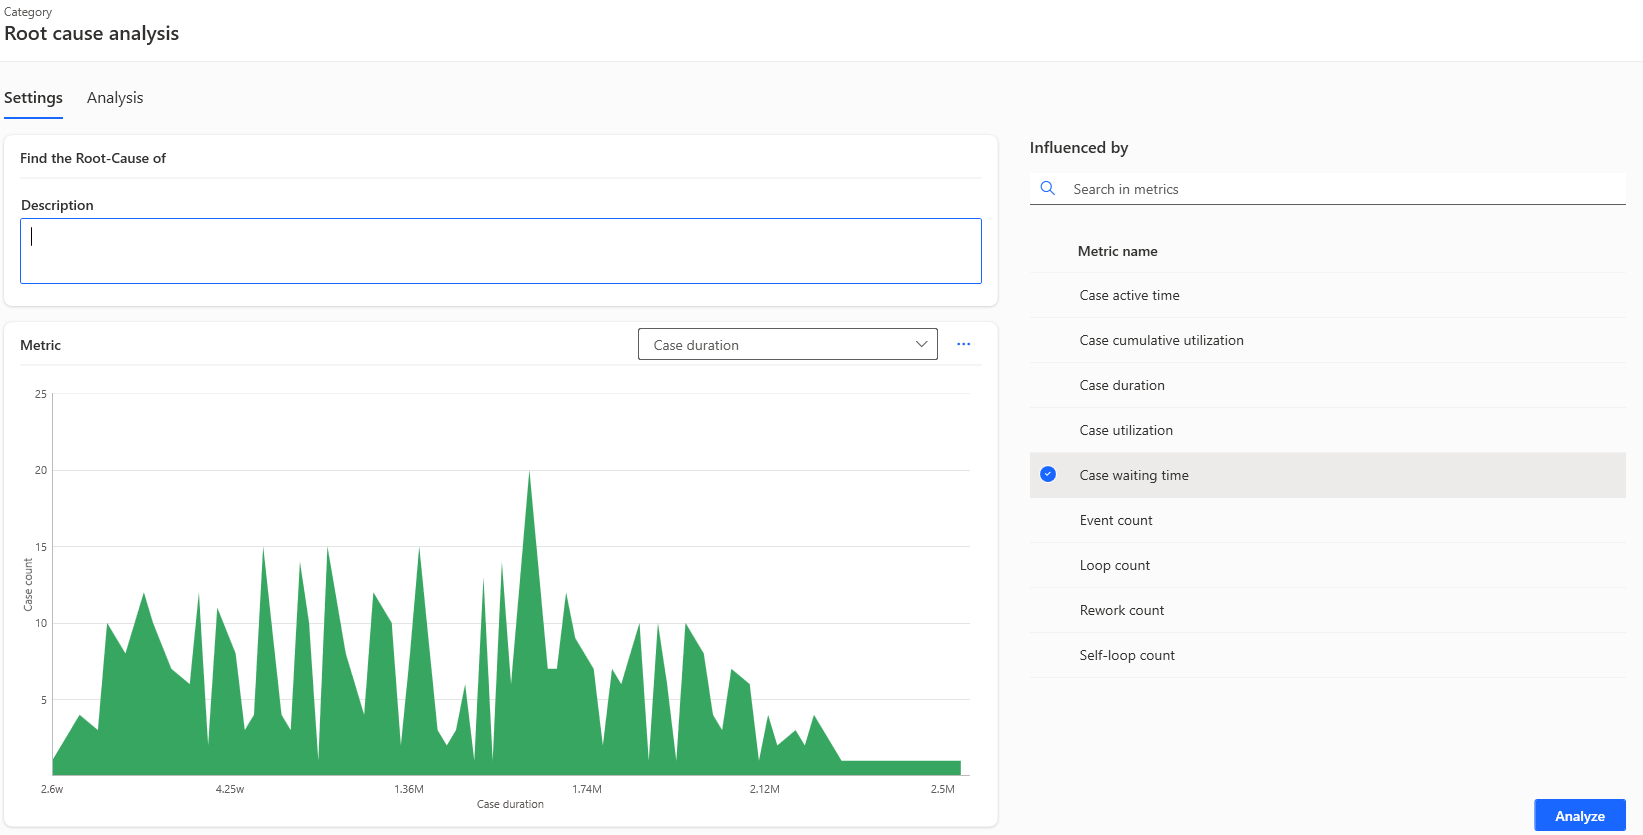
\includegraphics[width=\textwidth]{imgMicrosoft/SecondaSimulazione/RootCauseAnalysisSettingsSimulazione2.png}
    \caption{Impostazioni dell'analisi delle cause radice}
    \label{fig:root-cause-analysis-settings}
\end{figure}
La schermata di "Root Cause Analysis" è uno strumento fondamentale per identificare e comprendere le cause principali che influenzano determinati risultati o metriche nel processo simulato. In questo caso, la schermata si concentra sulla durata dei casi, con l'obiettivo di determinare quali fattori influenzano maggiormente il tempo complessivo necessario per completare un ciclo di attività.\\
Nella schermata visualizzata, è possibile osservare che la metrica selezionata per l'analisi è la "Case duration" (durata dei casi). Questa scelta è significativa, poiché la durata dei casi è un indicatore chiave dell'efficienza del processo produttivo.\\
La grafica a barre mostra la distribuzione dei casi in base alla loro durata, offrendo una panoramica visiva di come si differenziano i tempi di completamento tra i vari casi. La distribuzione è varia, con una presenza significativa di casi che rientrano in intervalli di durata specifici, indicando possibili aree di interesse per un'analisi più approfondita.\\
\begin{figure}[H]
    \centering
    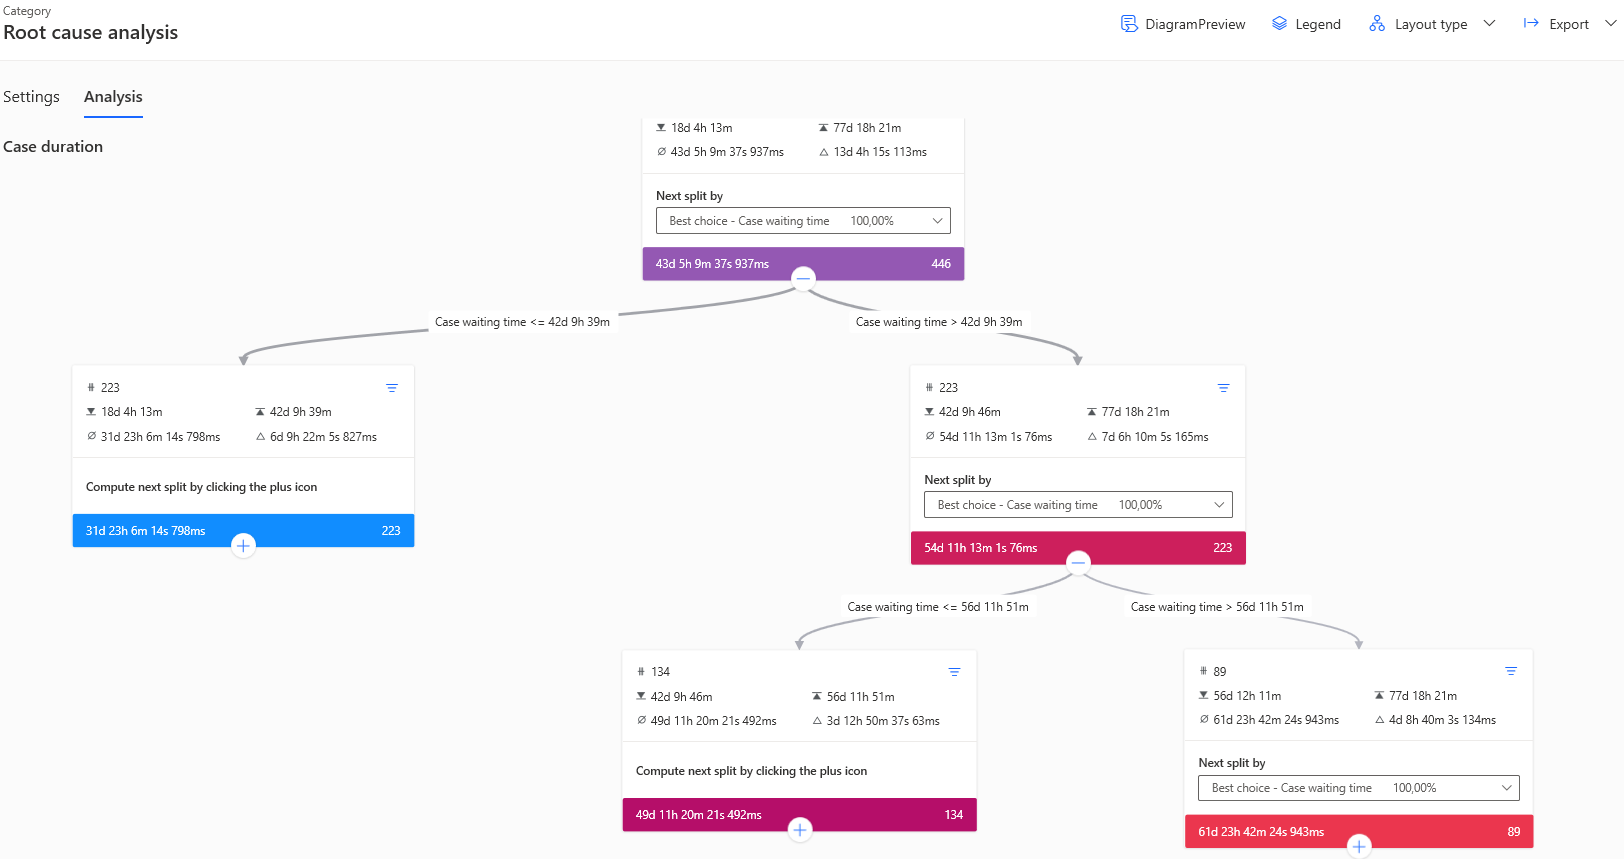
\includegraphics[width=\textwidth]{imgMicrosoft/SecondaSimulazione/RootCauseAnalysisSimulazione2.png}
    \caption{Analisi delle cause radice}
    \label{fig:root-cause-analysis}
\end{figure}
La schermata di analisi presenta una struttura ad albero che parte da una suddivisione iniziale basata sul tempo di attesa dei casi (Case waiting time). Questo parametro è stato utilizzato per separare i casi in base alla loro durata totale, evidenziando come il tempo di attesa contribuisca alla durata complessiva.\\
L'analisi mette in luce come il tempo di attesa sia un fattore critico che influisce in modo sostanziale sulla durata dei casi. I casi con un tempo di attesa più lungo tendono ad avere una durata complessiva molto maggiore, indicando che ridurre i tempi di attesa potrebbe portare a un miglioramento significativo dell'efficienza del processo.\\
Il diagramma ad albero visualizza chiaramente come i casi vengono influenzati dal tempo di attesa, permettendo di identificare i punti esatti del processo dove si accumulano i ritardi. Questo tipo di analisi è fondamentale per identificare le aree del processo che necessitano di interventi per ridurre i tempi di attesa e, di conseguenza, migliorare la produttività complessiva.\\

\subsubsection{Variants}
\begin{figure}[H]
    \centering
    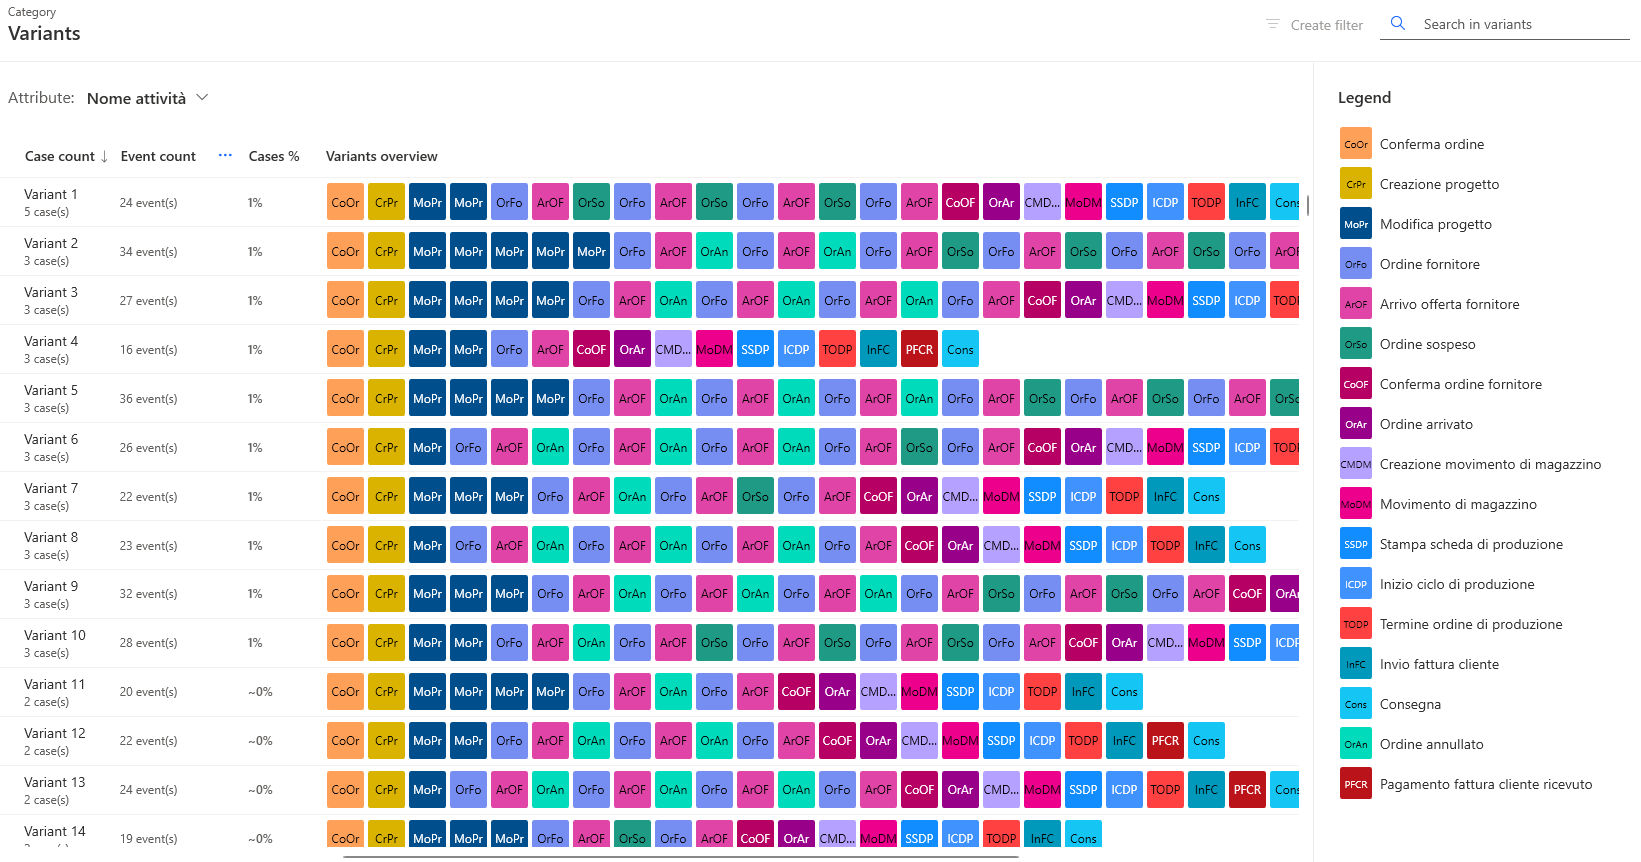
\includegraphics[width=\textwidth]{imgMicrosoft/SecondaSimulazione/VariantsSimulazione2.png}
    \caption{Varianti}
    \label{fig:variants}
\end{figure}
La schermata delle varianti del processo mostra le diverse sequenze di attività che si verificano all'interno del flusso di lavoro simulato. Ogni variante rappresenta un percorso alternativo che un caso può seguire, riflettendo la flessibilità e la complessità del processo produttivo.\\
Nella schermata sono rappresentate numerose varianti, ciascuna con una diversa combinazione e sequenza di attività. Ogni variante è identificata da un numero di casi e di eventi associati, mostrando come il processo possa divergere in molteplici direzioni. Anche se ogni variante rappresenta solo una piccola percentuale del totale dei casi (1\% o meno), la loro presenza indica un'ampia variabilità nei percorsi seguiti.\\
Le prime varianti, come Variante 1 e Variante 2, presentano una combinazione di attività come "Conferma ordine", "Creazione progetto", e "Modifica progetto", che sono tipicamente seguite da attività legate agli ordini dei fornitori come "Ordine fornitore" e "Arrivo offerta fornitore". Questo riflette un flusso di lavoro abbastanza standard, dove il progetto è creato e modificato prima di passare alla gestione degli ordini.\\
Altre varianti, come Variante 7 e Variante 8, includono attività aggiuntive come "Ordine sospeso", "Ordine annullato", e "Movimento di magazzino", indicando che alcuni casi subiscono interruzioni o modifiche significative durante il processo, portando a deviazioni dal flusso standard.\\
Alcune varianti più complesse, come quelle numerate verso la fine della lista, mostrano sequenze lunghe e intricate di attività, con una combinazione di passaggi che coinvolgono molte fasi della gestione degli ordini, della produzione e della consegna. Queste varianti indicano processi più complessi, potenzialmente dovuti a esigenze specifiche del cliente, problemi operativi, o modifiche post-ordine.\\
La presenza di molte varianti con sequenze uniche di attività suggerisce un alto livello di flessibilità nel processo, ma potrebbe anche indicare potenziali inefficienze o complessità gestionali. Varianti che includono attività come "Ordine sospeso" o "Ordine annullato" potrebbero evidenziare problemi ricorrenti che richiedono attenzione per migliorare l'efficienza del processo.\\
La rappresentazione grafica delle varianti offre una visione immediata della diversità dei percorsi seguiti nel processo. La presenza di molte varianti con poche occorrenze potrebbe indicare che il processo è soggetto a numerose eccezioni o che è altamente personalizzabile. Tuttavia, un numero elevato di varianti può complicare la gestione del processo e richiedere una standardizzazione maggiore per migliorare la coerenza e ridurre i costi operativi.\\

\subsection{Terza simulazione}
Il file CSV è stato creato mediante uno script Python che simula una serie di attività relative alla produzione e alla gestione degli ordini di prodotti. Inoltre, per la simulazione dei dati, sono stati presi in considerazione anche i dati estratti manualmente da un database di un sistema gestionale.
\subsubsection{Regole di simulazione}
\custombold{Impostazione delle date iniziali}\\
Ogni ciclo di attività inizia con la prima attività programmata tra il 1 gennaio 2019 e il 31 dicembre 2020.\\
\custombold{Definizione delle tipologie di prodotti}\\
Viene creata una lista di 30 tipi di scarpe, denominate "Scarpe tipo 1" fino a "Scarpe tipo 30".\\
\custombold{Definizione delle attività e delle durate}\\
Sono state definite 17 attività, ciascuna con un ID unico e una durata variabile. Le durate delle attività sono espresse in minuti o giorni, a seconda dell'attività specifica.\\
\custombold{Generazione di un ciclo di attività per prodotto}\\
Per ciascun prodotto, viene generato un ciclo di attività che segue le seguenti regole:
\begin{itemize}
    \item \custombold{attività obbligatorie}: alcune attività avvengono in un ordine fisso. Ad esempio, "Conferma ordine" è sempre seguita da "Creazione progetto";
    \item \custombold{modifica del progetto}: un numero casuale di modifiche al progetto (da 1 a 5) può essere aggiunto dopo la creazione del progetto;
    \item \custombold{gestione degli ordini fornitore}: un numero casuale (da 1 a 3) di cicli di gestione ordini fornitore può essere inserito, ognuno dei quali può includere attività come "Ordine fornitore", "Arrivo offerta fornitore", "Ordine annullato" o "Ordine sospeso";
    \item \custombold{produzione}: vengono aggiunte attività relative alla produzione, come "Stampa scheda di produzione", "Inizio ciclo di produzione" e "Termine ordine di produzione";
    \item \custombold{attività non necessarie}: possono essere inserite attività opzionali come "Controllo qualità non necessario" (20\% di probabilità) e "Ri-lavorazione non necessaria" (10\% di probabilità);
    \item \custombold{consegna}: dopo la produzione, viene aggiunta l'attività di "Consegna".
\end{itemize}
\custombold{Generazione dei timestamp}\\
Ogni attività riceve un timestamp generato casualmente basato su un intervallo di tempo definito per quella specifica attività.\\
\custombold{Ciclo di generazione dei dati}\\
Il numero di prodotti varia tra 300 e 500, determinato casualmente. Per ogni prodotto, viene generato un ciclo di attività completo, assicurandosi che tutte le attività obbligatorie siano inserite nel corretto ordine e che le attività casuali siano distribuite come specificato.\\
\custombold{Mischiamento casuale delle righe del file CSV}\\
È stato utilizzato un algoritmo per mischiare in modo casuale le righe del file CSV. L'algoritmo legge il file CSV originale e separa l'intestazione dai dati. Successivamente, le righe dei dati vengono mescolate casualmente mantenendo intatta l'intestazione. Infine, il nuovo file CSV, con le righe mescolate, viene salvato in un file di output. Questo processo assicura che i dati siano riorganizzati in modo casuale senza alterare la struttura del file CSV.

\subsubsection{Process map}
\begin{figure}[H]
    \centering
    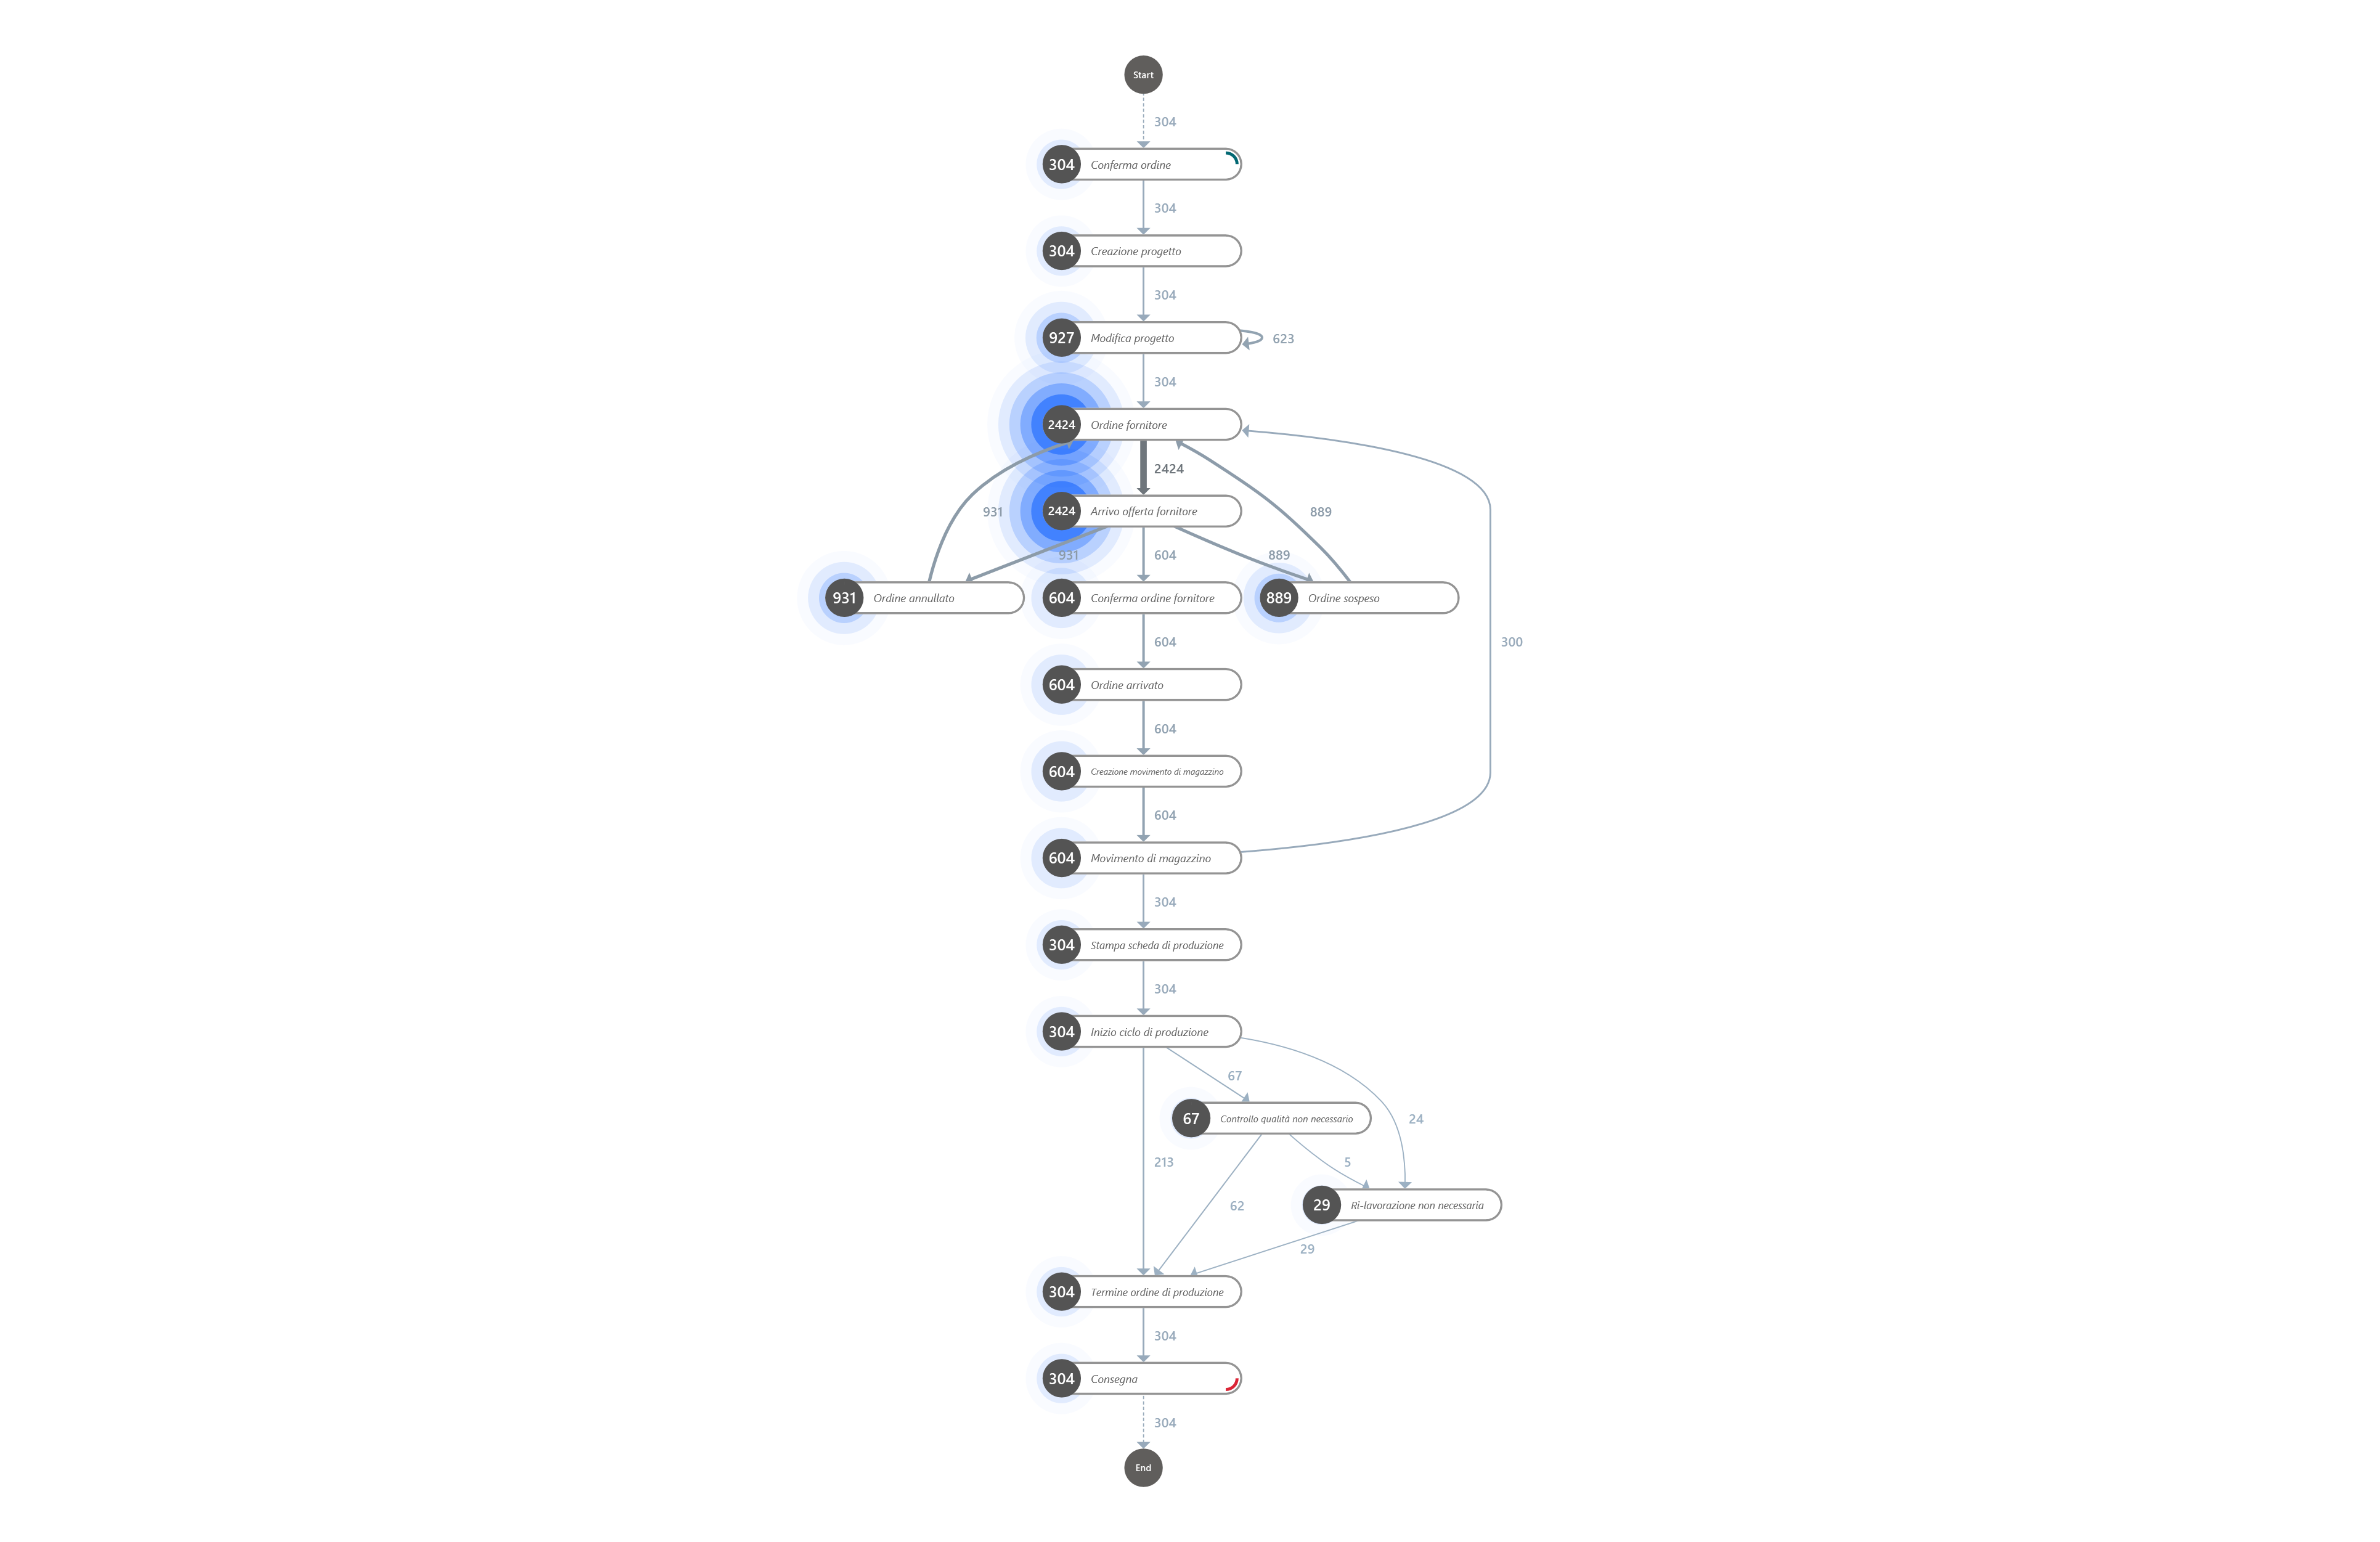
\includegraphics[width=\textwidth]{imgMicrosoft/TerzaSimulazione/ProcessMapSimulazione3.png}
    \caption{Mappa del processo}
    \label{fig:process-map}
\end{figure}
La mappa visualizza la sequenza delle attività, evidenziando i collegamenti, le diramazioni e le attività opzionali che si verificano all'interno del ciclo di produzione e gestione degli ordini.\\
Il processo inizia con l'attività "Conferma ordine", seguita da "Creazione progetto". Queste sono attività obbligatorie per ogni ciclo, come indicato dalle regole di simulazione. Successivamente, il processo può includere uno o più cicli di "Modifica progetto", che riflettono la possibilità di revisioni del progetto prima di procedere con l'ordine al fornitore.\\
La fase di gestione degli ordini al fornitore è rappresentata da diverse attività chiave, tra cui "Ordine fornitore", "Arrivo offerta fornitore", e può includere eventuali interruzioni come "Ordine annullato" e "Ordine sospeso". Queste varianti sono chiaramente rappresentate nella mappa, mostrando la flessibilità del processo e le decisioni che possono portare a percorsi alternativi.\\
Dopo la conferma dell'ordine da parte del fornitore, il processo procede verso la fase di produzione. Questa include attività come "Stampa scheda di produzione", "Inizio ciclo di produzione" e "Termine ordine di produzione". Oltre alle attività obbligatorie, la simulazione include attività non necessarie ma possibili, come "Controllo qualità non necessario" e "Ri-lavorazione non necessaria". La mappa evidenzia chiaramente come queste attività opzionali si inseriscano nel flusso di lavoro, indicando potenziali aree di inefficienza.\\
Il processo si conclude con la "Consegna" del prodotto, che è l'ultima attività rappresentata nella mappa. Ogni passaggio del processo è chiaramente delineato, mostrando sia i percorsi lineari che le deviazioni possibili.\\
La mappa mostra una struttura ben organizzata con percorsi chiari e collegamenti logici tra le attività. Le bolle di dimensioni diverse e le connessioni tra di esse riflettono la frequenza e l'importanza delle transizioni, permettendo di identificare facilmente le attività principali e i punti di decisione critici.\\
Un aspetto notevole è la presenza di attività opzionali, come il "Controllo qualità non necessario" e la "Ri-lavorazione non necessaria", che, pur essendo poco frequenti, rappresentano potenziali colli di bottiglia e inefficienze nel processo. Queste attività, essendo opzionali, si verificano con una probabilità inferiore e sono chiaramente visualizzate come deviazioni dal percorso principale.\\
La mappa riflette accuratamente la complessità del processo produttivo, inclusa la possibilità di modifiche al progetto, annullamenti o sospensioni degli ordini, e attività opzionali.\\
La mappa di processo della terza simulazione offre una rappresentazione dettagliata e coerente del flusso di lavoro simulato, evidenziando sia le attività obbligatorie che quelle opzionali. La struttura della mappa riflette accuratamente le regole di simulazione, offrendo una visione chiara delle diverse possibilità all'interno del ciclo di produzione e gestione degli ordini.

\subsubsection{Statistics case overview}
\begin{figure}[H]
    \centering
    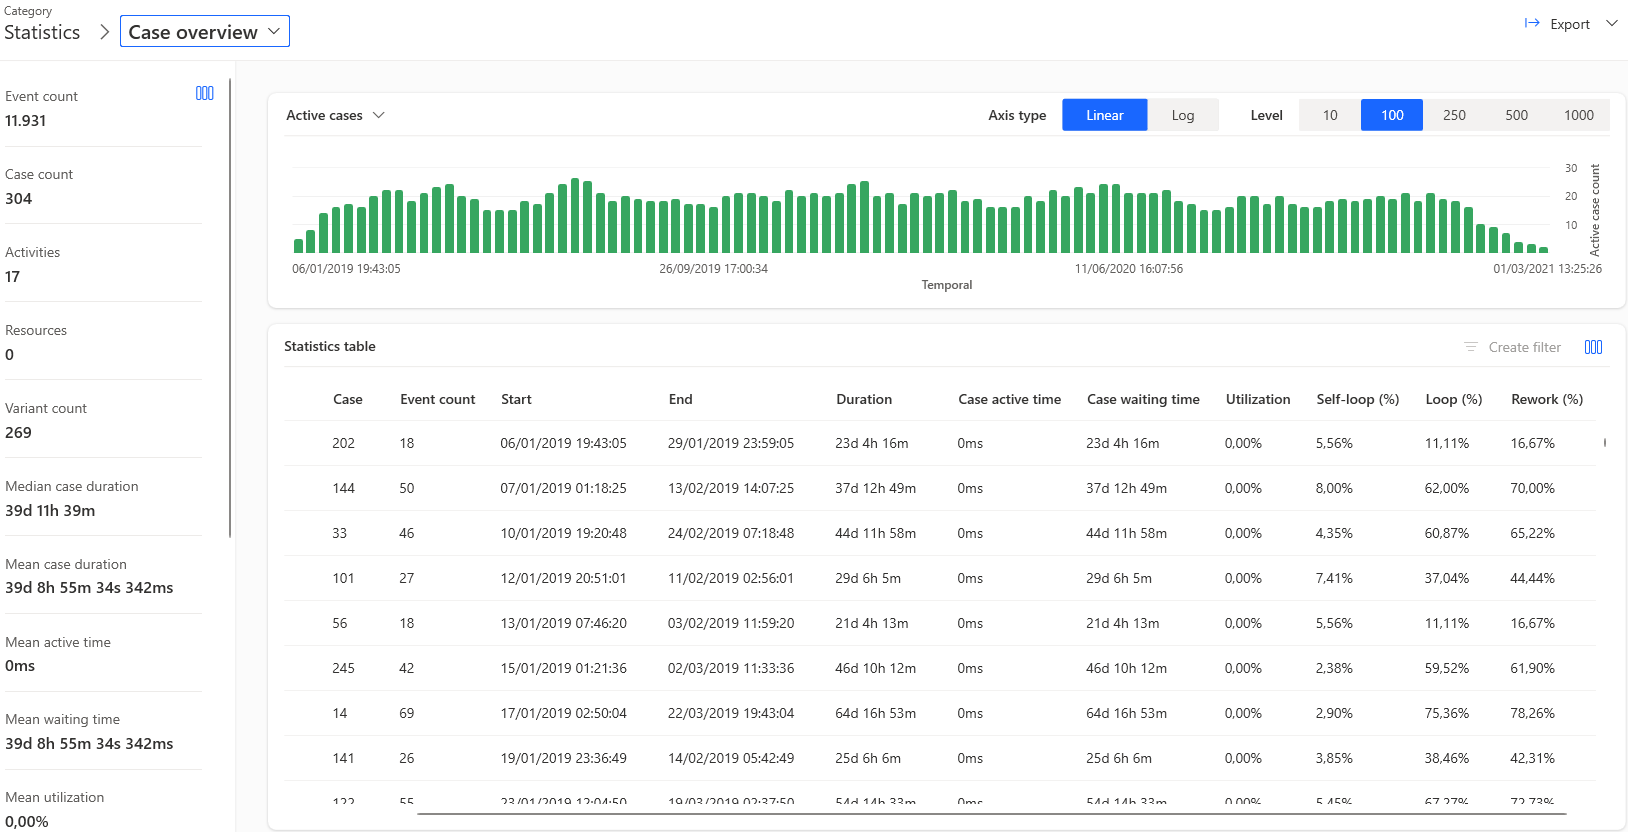
\includegraphics[width=\textwidth]{imgMicrosoft/TerzaSimulazione/StatisticsCaseOverviewSimulazione3.png}
    \caption{Statistiche dei casi}
    \label{fig:statistics-case-overview}
\end{figure}
La schermata di panoramica dei casi fornisce un'analisi dettagliata delle attività produttive e gestionali relative a 304 casi simulati. Questa simulazione rappresenta un flusso di lavoro complesso con 17 diverse attività coinvolte e una significativa variabilità nei tempi di completamento e nelle caratteristiche operative dei casi. L'obiettivo di questa analisi è di comprendere meglio la distribuzione delle durate dei casi, il numero di eventi, i tempi di attesa e altri parametri chiave.\\
Il numero totale di eventi registrati è di 11.931 distribuiti su 304 casi. La durata mediana di un caso è di 39 giorni, 11 ore e 39 minuti, mentre la durata media dei casi è di 39 giorni, 8 ore, 55 minuti e 34 secondi, con una lieve variabilità indicata dalla deviazione standard.\\
La schermata evidenzia una distribuzione temporale dei casi attivi, che varia nel tempo con un picco centrale. Questo potrebbe riflettere un ciclo produttivo caratterizzato da una fase centrale di maggiore attività, seguita da un progressivo decremento del numero di casi attivi.\\
Il tempo di attesa medio per i casi coincide esattamente con la durata media dei casi, indicando che non vi è tempo attivo registrato nei dati. Questo suggerisce che le attività siano distribuite nel tempo senza intervalli di inattività significativa, oppure che il tempo di inattività non sia stato catturato nei dati.\\
L'utilizzo medio riportato è 0,00\%, suggerendo che le risorse non sono state monitorate o che il focus della simulazione non includeva la gestione delle risorse. Questo aspetto limita l'analisi all'efficienza temporale del processo senza considerare l'efficienza delle risorse.\\
L'analisi mostra che ci sono casi con una percentuale significativa di "self-loop" e "rework". Ad esempio:
\begin{itemize}
    \item il caso 144 ha un 8,00\% di self-loop e un 70,00\% di rework, indicando che questo caso ha subito numerose iterazioni o revisioni. Questo potrebbe suggerire problemi nella fase di produzione o nelle fasi precedenti che hanno richiesto modifiche e aggiustamenti;
    \item il caso 245, con una durata di 46 giorni, 10 ore e 12 minuti, presenta un 61,90\% di rework e un 2,38\% di self-loop, indicando che una parte significativa del processo è stata ripetuta, portando a un allungamento della durata complessiva.
\end{itemize}
Il grafico degli "Active cases" mostra come il numero di casi attivi varia nel tempo. Il picco nel numero di casi attivi potrebbe essere indicativo di un periodo di alta domanda o di una fase specifica del ciclo produttivo con maggiore intensità operativa.\\
Verso la fine del periodo di analisi, si osserva una diminuzione graduale del numero di casi attivi, il che può indicare un rallentamento nelle operazioni o la conclusione della maggior parte dei cicli produttivi.\\
La schermata di panoramica dei casi della terza simulazione offre una visione completa della durata e della complessità dei casi all'interno del processo produttivo simulato. La presenza di numerose varianti con self-loop e rework elevati suggerisce la possibilità di inefficienze che potrebbero essere affrontate per migliorare l'efficienza complessiva del processo.

\subsubsection{Statistics per nome attività}
\begin{figure}[H]
    \centering
    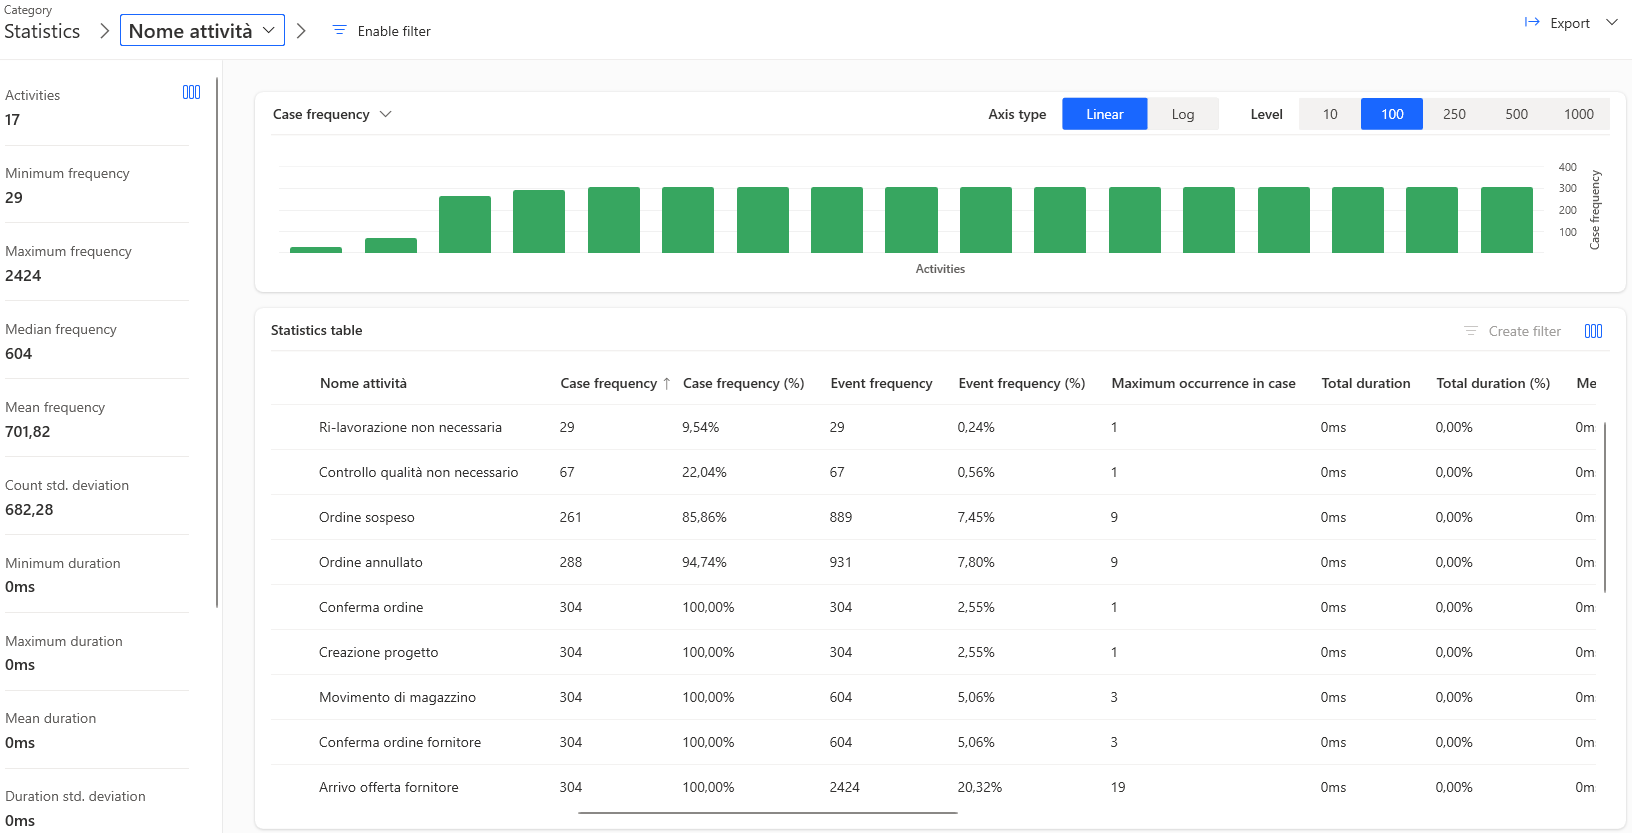
\includegraphics[width=\textwidth]{imgMicrosoft/TerzaSimulazione/StatisticsNomeAttivitaSimulazione3.png}
    \caption{Statistiche per nome attività}
    \label{fig:statistics-nome-attività}
\end{figure}
La schermata delle statistiche per "Nome attività" fornisce un'analisi dettagliata della frequenza con cui ciascuna attività si verifica all'interno del processo simulato. Questa simulazione, che coinvolge 304 casi e 17 attività diverse, riflette la complessità e la varietà dei flussi di lavoro nella gestione della produzione e degli ordini.\\
Le attività all'interno del processo mostrano una distribuzione di frequenza che varia significativamente. La frequenza minima è di 29 occorrenze, mentre la massima è di 2.424. La frequenza mediana delle attività è di 604, con una media di 701,82 e una deviazione standard di 682,28, suggerendo una distribuzione non uniforme delle attività. Attività con la frequenza più alta includono:
\begin{itemize}
    \item "Arrivo offerta fornitore" con 2.424 occorrenze, rappresenta il 20,32\% della frequenza totale degli eventi. Questa attività è centrale nel processo e si ripete più volte in ciascun caso, evidenziando l'importanza del dialogo e della gestione degli ordini con i fornitori;
    \item "Conferma ordine" e "Creazione progetto" con 304 occorrenze ciascuna (100\% dei casi), sono attività fondamentali e presenti in tutti i cicli, confermando il loro ruolo essenziale nel processo.
\end{itemize}
D'altra parte, le attività meno frequenti come "Ri-lavorazione non necessaria" e "Controllo qualità non necessario" con rispettivamente 29 e 67 occorrenze, rappresentano azioni opzionali che si verificano in una minoranza di casi, indicando aree potenziali di inefficienza o di controlli aggiuntivi che non sempre risultano necessari.\\
La "Event frequency" conferma ulteriormente l'importanza delle attività più frequenti. Per esempio:
\begin{itemize}
    \item "Ordine annullato" con 931 eventi e una frequenza di 7,80\%, suggerisce che una parte significativa degli ordini può essere soggetta a cancellazioni, un aspetto critico che potrebbe avere impatti significativi sulla produttività e sui tempi di completamento dei casi;
    \item "Ordine sospeso" con 889 eventi, rappresenta un'altra attività ricorrente che può causare ritardi nel flusso di lavoro.
\end{itemize}
Le attività con frequenze elevate indicano passaggi obbligatori e ripetuti che sono fondamentali per il completamento del processo. Tuttavia, la presenza di attività opzionali come il "Controllo qualità non necessario" o la "Ri-lavorazione non necessaria" suggerisce che vi siano opportunità di miglioramento per ridurre le operazioni ridondanti e ottimizzare il flusso di lavoro.\\
L'alta frequenza di eventi come "Ordine annullato" o "Ordine sospeso" può indicare problematiche ricorrenti nel processo di gestione degli ordini che potrebbero richiedere interventi per minimizzare i ritardi e le cancellazioni.\\
La schermata delle statistiche per "Nome attività" nella terza simulazione evidenzia la centralità di alcune attività e l'importanza delle interazioni con i fornitori, nonché la gestione e la modifica degli ordini. Le attività meno frequenti e opzionali rappresentano potenziali aree di inefficienza, mentre l'alta frequenza di ordini sospesi e annullati indica possibili problemi nel flusso di lavoro che potrebbero beneficiare di ulteriore analisi e ottimizzazione.\\

\subsubsection{Edge statistics}
\begin{figure}[H]
    \centering
    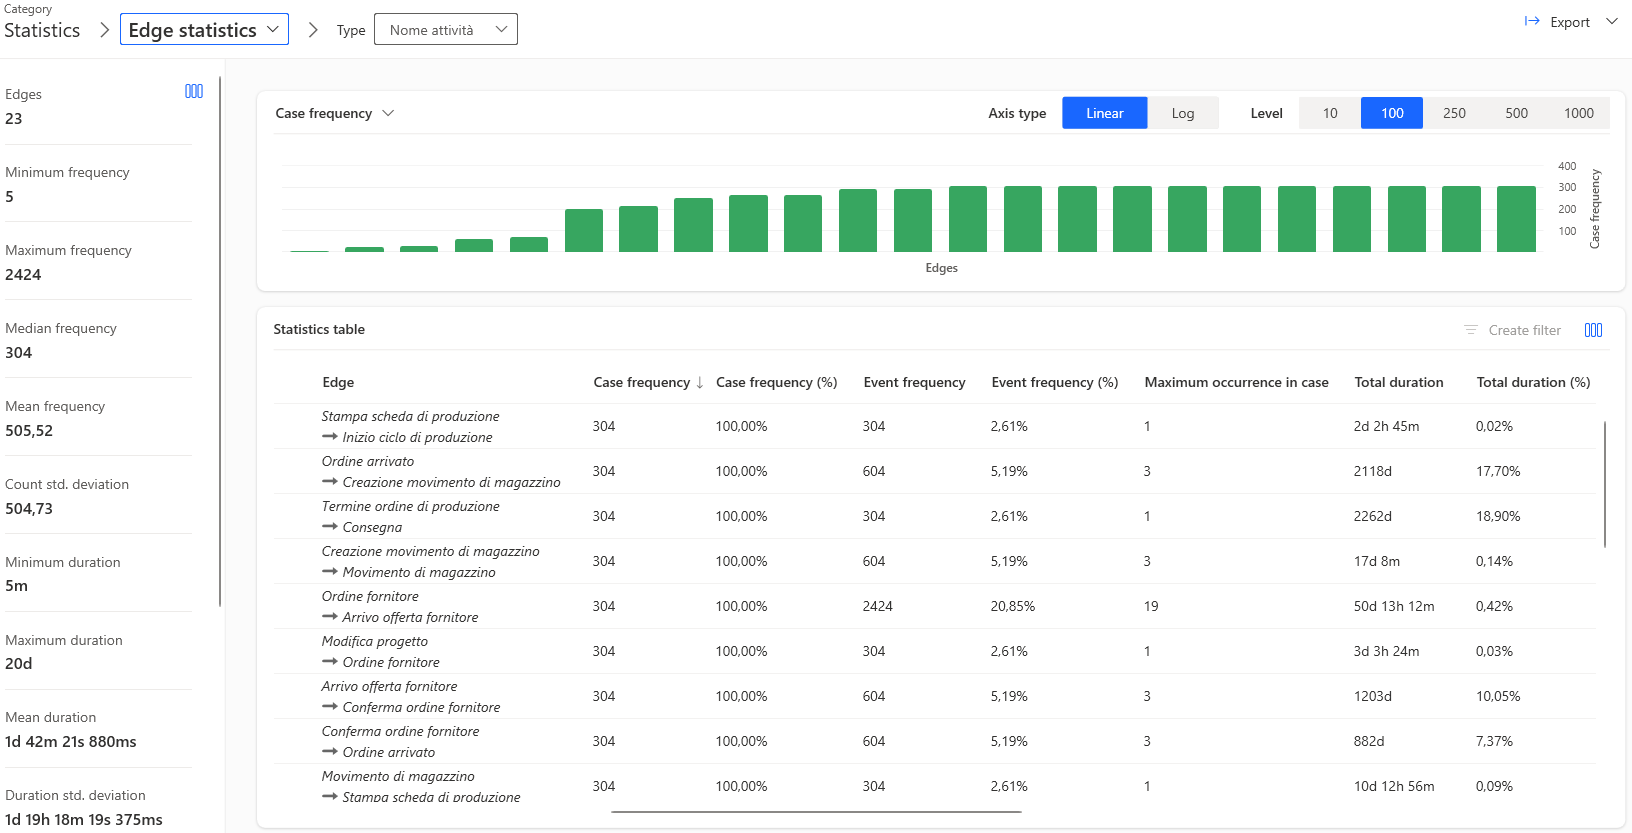
\includegraphics[width=\textwidth]{imgMicrosoft/TerzaSimulazione/StatisticsEdgeStatisticsSimulazione3.png}
    \caption{Statistiche dei collegamenti}
    \label{fig:edge-statistics}
\end{figure}
La schermata delle statistiche dei collegamenti ("Edge statistics") analizza le transizioni tra le diverse attività all'interno del processo produttivo simulato. Ogni collegamento rappresenta un passaggio tra due attività, evidenziando quante volte si verifica la transizione e la sua durata complessiva.\\
Nella schermata sono riportati 23 collegamenti principali tra le attività, con una frequenza minima di 5 e una massima di 2.424. La frequenza mediana dei collegamenti è di 304, con una media di 505,52 e una deviazione standard di 504,73. Questi dati indicano una notevole variabilità nella frequenza dei collegamenti, suggerendo che alcune transizioni sono molto più comuni di altre. I collegamenti più frequenti includono:
\begin{itemize}
    \item "Ordine fornitore" $\rightarrow$ "Arrivo offerta fornitore" con 2.424 occorrenze, rappresenta il 20,85\% della frequenza totale degli eventi. Questa transizione riflette una parte cruciale del processo di gestione degli ordini e rappresenta un punto focale nel flusso di lavoro;
    \item "Ordine arrivato" $\rightarrow$ "Creazione movimento di magazzino" con 604 occorrenze, rappresenta il 5,19\% della frequenza totale. Questo passaggio è legato alla gestione dei materiali dopo la ricezione degli ordini e precede il processo di produzione.
\end{itemize}
Le durate complessive delle transizioni variano significativamente, con alcune che occupano una porzione rilevante del tempo complessivo del processo. I collegamenti più lunghi includono:
\begin{itemize}
    \item "Ordine fornitore" $\rightarrow$ "Arrivo offerta fornitore", con una durata totale di 1.203 giorni, rappresenta il 10,05\% della durata complessiva del processo. Questa transizione ha un impatto significativo sui tempi totali, indicando un possibile collo di bottiglia;
    \item "Termine ordine di produzione" $\rightarrow$ "Consegna", con una durata complessiva di 2.262 giorni, rappresenta il 18,90\% della durata totale del processo. Questo dato suggerisce che il tempo impiegato tra la fine della produzione e la consegna è particolarmente rilevante per la durata complessiva del ciclo produttivo.
\end{itemize}
Altri collegamenti con un impatto importante includono "Arrivo offerta fornitore" $\rightarrow$ "Conferma ordine fornitore", con una durata complessiva di 882 giorni e un impatto del 7,37\% sul tempo totale del processo.\\
I collegamenti meno frequenti, come "Modifica progetto" $\rightarrow$ "Ordine fornitore" (304 occorrenze) e "Movimento di magazzino" $\rightarrow$ "Stampa scheda di produzione" (304 occorrenze), rappresentano transizioni che non accadono in tutti i casi ma che comunque contribuiscono al completamento del processo. Queste transizioni sono importanti per i flussi di lavoro specifici e per la gestione dei materiali e delle risorse.\\
Le durate di alcune transizioni, come "Stampa scheda di produzione" $\rightarrow$ "Inizio ciclo di produzione", sono relativamente brevi rispetto ad altre. Questo suggerisce che, una volta che la produzione è avviata, il processo procede in modo efficiente fino alla conclusione, senza ritardi significativi in queste fasi.\\
La schermata delle statistiche dei collegamenti nella terza simulazione mostra una chiara distribuzione delle transizioni tra le attività chiave del processo produttivo. Le transizioni tra "Ordine fornitore" e "Arrivo offerta fornitore" sono le più frequenti, indicando che la gestione degli ordini rappresenta una parte cruciale e ripetitiva del flusso di lavoro. Tuttavia, la durata significativa di alcuni collegamenti, come quello tra "Ordine fornitore" e "Arrivo offerta fornitore", suggerisce aree di possibile ottimizzazione per ridurre i tempi di attesa e migliorare l'efficienza complessiva.

\subsubsection{Statistiche prodotto}
\begin{figure}[H]
    \centering
    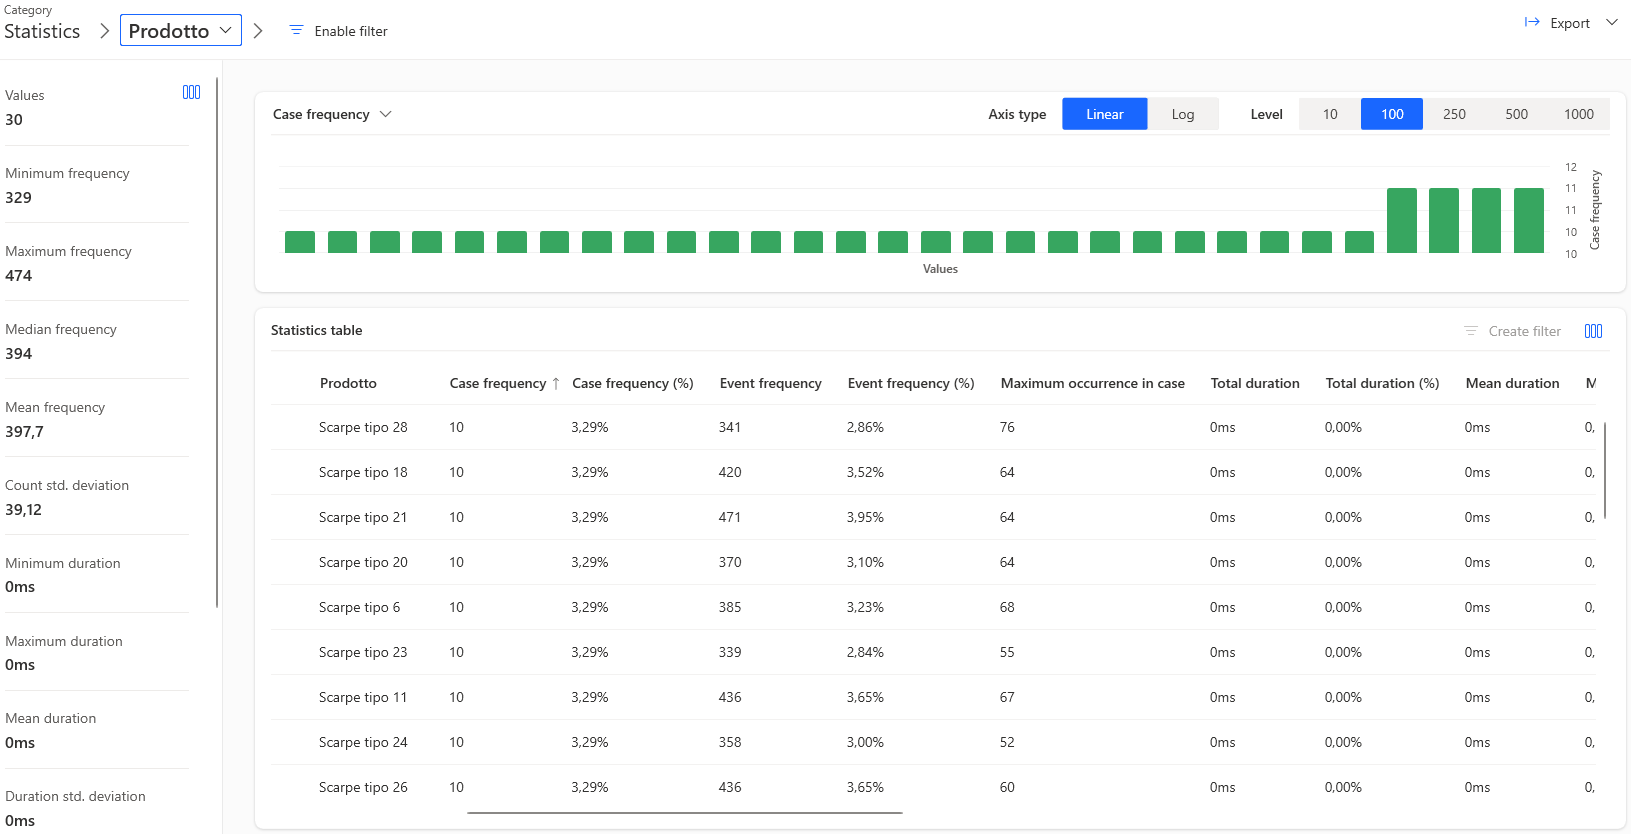
\includegraphics[width=\textwidth]{imgMicrosoft/TerzaSimulazione/StatisticsProdottoSimulazione3.png}
    \caption{Statistiche dei prodotti}
    \label{fig:statistics-prodotti}
\end{figure}
La schermata delle statistiche per prodotto fornisce un'analisi dettagliata della frequenza con cui i vari tipi di scarpe, definiti come "Scarpe tipo 1" fino a "Scarpe tipo 30", sono coinvolti nel processo produttivo simulato.\\
Nella simulazione, il numero di casi per ciascun tipo di scarpa varia leggermente, ma è distribuito in modo relativamente uniforme. La frequenza minima registrata è di 329 casi, mentre la massima è di 474. La frequenza mediana è 394, con una media di 397,7 e una deviazione standard di 39,12. Questi dati indicano una distribuzione abbastanza equilibrata delle attività tra i vari prodotti. Alcuni dei prodotti con la frequenza più alta includono:
\begin{itemize}
    \item "Scarpe tipo 21" con 471 eventi, che rappresenta il 3,95\% dell'event frequency totale. Questo prodotto ha una frequenza leggermente superiore rispetto ad altri, suggerendo che potrebbe essere uno dei modelli più popolari o che richiede più attenzione nel processo.
    \item "Scarpe tipo 18" e "Scarpe tipo 6" con 420 e 385 eventi rispettivamente, rappresentano anche una parte significativa dell'attività, con frequenze del 3,52\% e 3,23\% rispettivamente.
\end{itemize}
D'altra parte, alcuni prodotti come "Scarpe tipo 28" e "Scarpe tipo 23" hanno una frequenza leggermente inferiore, ma comunque comparabile con gli altri, con 341 e 339 eventi rispettivamente.\\
È importante notare che, nonostante la variazione nella frequenza degli eventi per ciascun prodotto, la durata totale degli eventi riportata è 0ms per tutti i prodotti. Questo suggerisce che nella simulazione non è stato considerato o registrato il tempo necessario per completare ogni evento, limitando così la possibilità di valutare l'efficienza temporale del processo per ogni tipo di scarpa.\\
Le "maximum occurrence in case" variano leggermente tra i prodotti, ma queste differenze sono minime e indicano che la maggior parte dei prodotti segue un percorso simile attraverso il processo produttivo.\\
La distribuzione uniforme delle frequenze tra i vari tipi di scarpe suggerisce che il processo produttivo è bilanciato e che non vi sono modelli particolarmente privilegiati o trascurati nel flusso di lavoro. Tuttavia, la mancanza di dati sulla durata degli eventi limita la capacità di analizzare l'efficienza del tempo impiegato per ciascun prodotto.\\
La leggera variazione nelle frequenze degli eventi può comunque indicare differenze nelle richieste o nella complessità della produzione di alcuni modelli rispetto ad altri. Ad esempio, le "Scarpe tipo 21" con la frequenza di eventi più alta potrebbero rappresentare un modello con una domanda più elevata o con un processo produttivo più complesso.\\
La schermata delle statistiche per prodotto nella terza simulazione mostra una distribuzione abbastanza omogenea delle attività tra i vari modelli di scarpe, suggerendo un processo produttivo ben bilanciato. Tuttavia, la mancanza di dati sulla durata degli eventi rappresenta una limitazione significativa nell'analisi dell'efficienza temporale del processo.

\subsubsection{Root cause analysis}
\begin{figure}[H]
    \centering
    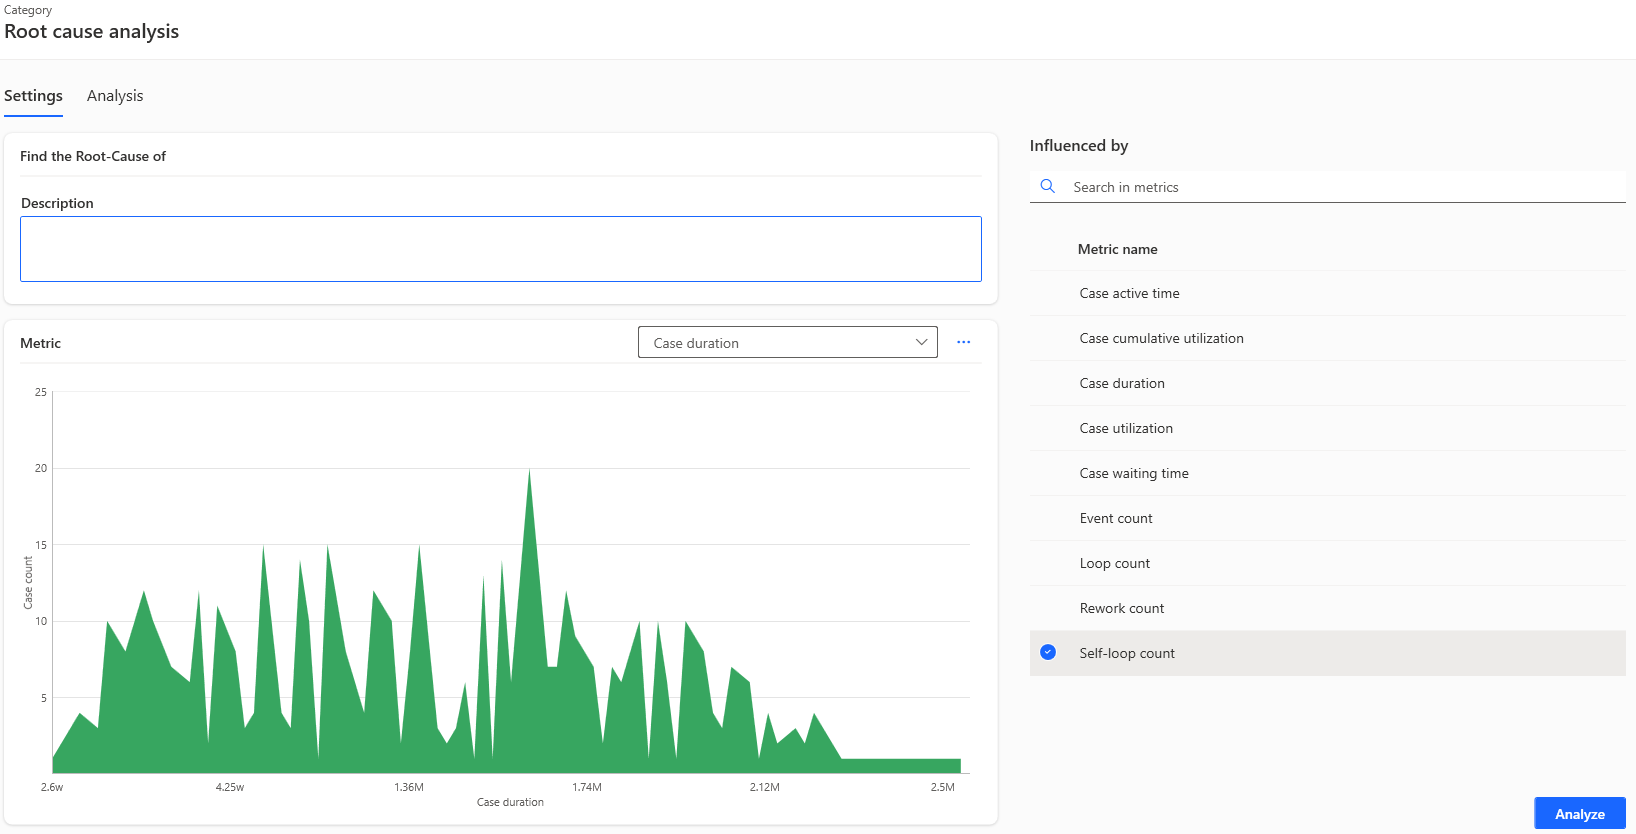
\includegraphics[width=\textwidth]{imgMicrosoft/TerzaSimulazione/RootCauseAnalysisSettingsSimulazione3.png}
    \caption{Impostazioni dell'analisi delle cause radice}
    \label{fig:root-cause-analysis-settings}
\end{figure}
La schermata di impostazioni per l'analisi delle cause radice fornisce gli strumenti necessari per identificare i fattori che influenzano le prestazioni del processo produttivo simulato. Questa sezione consente di selezionare una metrica chiave da analizzare, come la durata del caso, e di indagare su quali variabili o metodi influenzano maggiormente questa metrica.\\
In questa schermata, la metrica selezionata per l'analisi è Case duration (durata del caso), che rappresenta il tempo totale impiegato per completare un caso specifico all'interno del processo. Questa metrica è cruciale per comprendere l'efficienza operativa e identificare i colli di bottiglia o le inefficienze nel flusso di lavoro.\\
Il grafico mostrato nella schermata presenta la distribuzione della durata dei casi su un periodo che varia da 2,6 settimane a 2,5 mesi. La distribuzione non è uniforme, indicando che alcuni casi richiedono molto più tempo per essere completati rispetto ad altri. Questa variabilità nella durata potrebbe essere dovuta a diversi fattori, tra cui la complessità del prodotto, la necessità di ri-lavorazioni, la gestione degli ordini o le inefficienze nel processo.\\
La schermata offre una serie di metriche che possono essere analizzate per determinare il loro impatto sulla durata del caso. Queste includono:
\begin{itemize}
    \item \custombold{case active time}: il tempo attivo in cui il caso è effettivamente in corso;
    \item \custombold{case waiting time}: il tempo in cui il caso è in attesa tra le diverse fasi del processo;
    \item \custombold{loop count} e \custombold{self-loop count}: la frequenza con cui si ripetono cicli o attività specifiche;
    \item \custombold{rework count}: il numero di volte che un caso ha richiesto ri-lavorazioni.
\end{itemize}
Nell'analisi corrente, la metrica selezionata per l'influenza è Self-loop count (conteggio dei cicli ripetitivi), il che suggerisce che l'analisi si concentra su come la ripetizione di specifiche attività all'interno di un caso influisca sulla durata totale.\\
\begin{figure}[H]
    \centering
    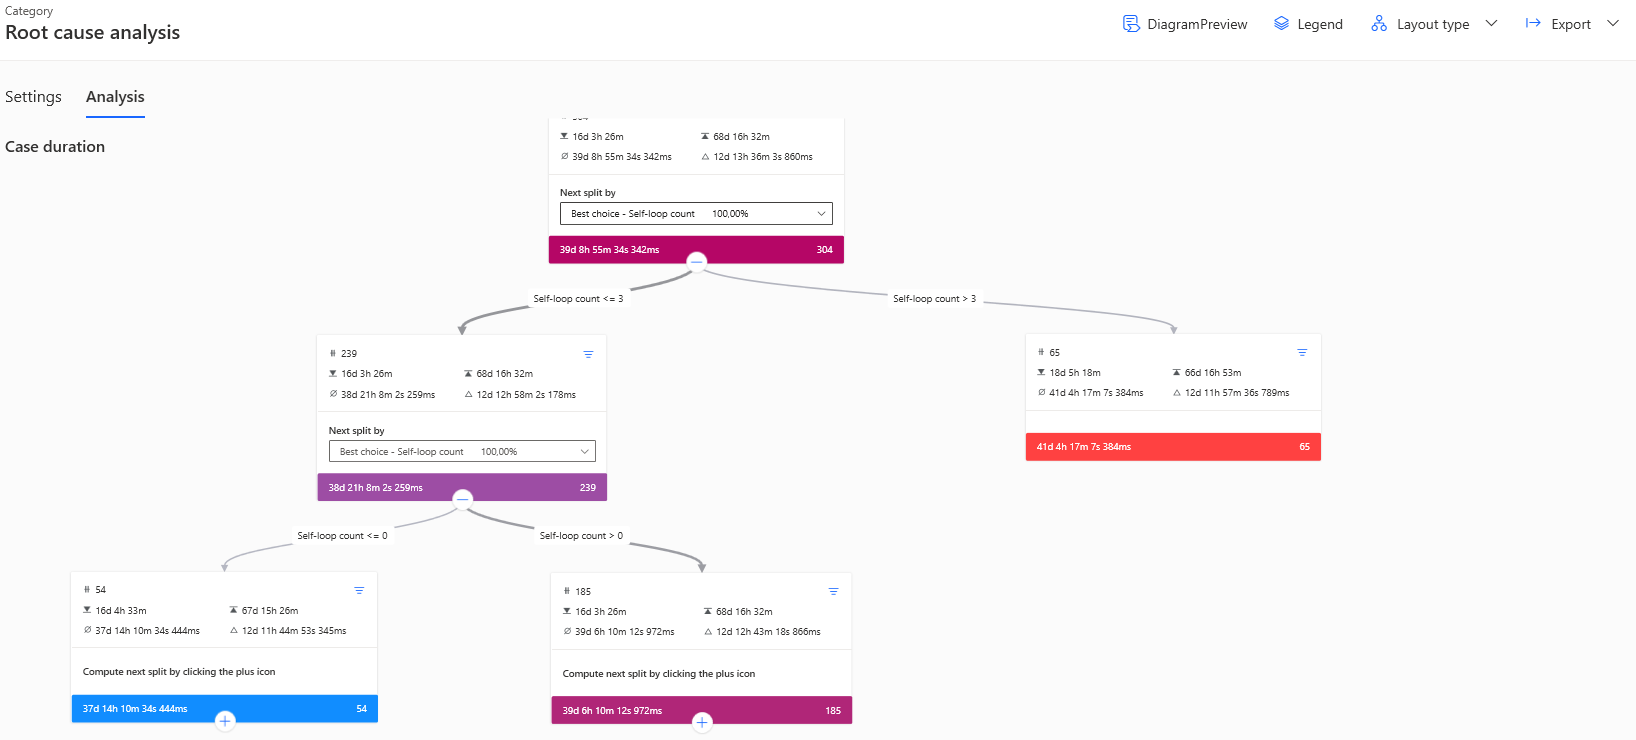
\includegraphics[width=\textwidth]{imgMicrosoft/TerzaSimulazione/RootCauseAnalysisSimulazione3.png}
    \caption{Analisi delle cause radice}
    \label{fig:root-cause-analysis}
\end{figure}
La schermata dell'analisi delle cause radice fornisce una rappresentazione visiva delle suddivisioni dei casi in base alla durata, con l'obiettivo di identificare i fattori principali che influenzano il tempo complessivo di completamento dei casi. Nella terza simulazione, l'analisi si concentra sulla durata dei casi e su come essa venga influenzata dal numero di "self-loop", ovvero la ripetizione di attività all'interno di un singolo caso.\\
Il diagramma suddivide i casi in base al numero di self-loop, evidenziando come questo parametro influisca sulla durata complessiva del caso.\\
L'analisi evidenzia chiaramente che il numero di self-loop è un fattore determinante per la durata complessiva dei casi. In particolare, l'aumento dei self-loop porta a un incremento del tempo necessario per completare il caso, con i casi che superano i tre self-loop che mostrano le durate più lunghe.\\
Questa correlazione suggerisce che per migliorare l'efficienza del processo, è essenziale concentrarsi sulla riduzione del numero di self-loop, possibilmente attraverso miglioramenti nel controllo qualità, una pianificazione più accurata, o l'ottimizzazione delle fasi di lavoro per evitare ripetizioni non necessarie.\\

\subsubsection{Variants}
\begin{figure}[H]
    \centering
    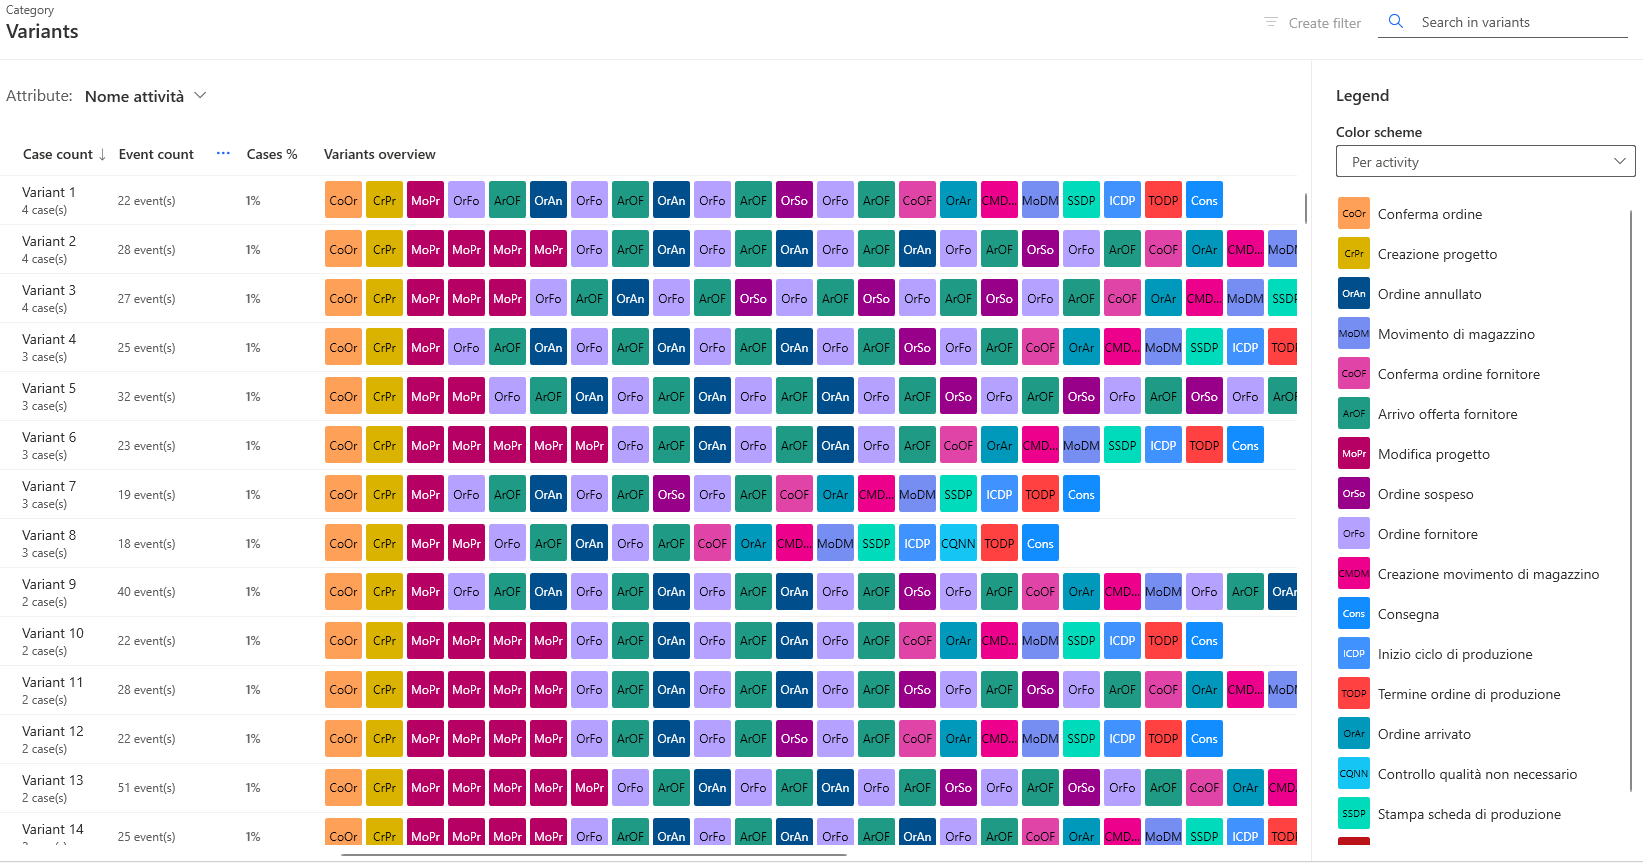
\includegraphics[width=\textwidth]{imgMicrosoft/TerzaSimulazione/VariantsSimulazione3.png}
    \caption{Variazioni}
    \label{fig:variants}
\end{figure}
La schermata delle varianti presenta una visione dettagliata delle diverse varianti dei processi che si verificano nella terza simulazione. Le varianti rappresentano i diversi percorsi seguiti dai casi durante il ciclo di produzione e gestione degli ordini. Ogni variante è caratterizzata da una sequenza unica di attività, e l'analisi di queste varianti è cruciale per comprendere la complessità e la variabilità del processo produttivo.\\
In questa simulazione, le varianti sono numerose e distribuite equamente, con ciascuna variante che rappresenta l'1\% dei casi totali. La schermata mostra 14 varianti principali, ciascuna con un numero di casi che varia da 2 a 4, e un numero di eventi associati che varia da 19 a 40.\\
Le attività all'interno delle varianti sono identificate tramite abbreviazioni colorate, come indicato nella legenda a destra della schermata. Questi colori facilitano l'identificazione delle attività principali e la comprensione delle differenze tra le varianti.\\
Ogni variante rappresenta una piccola percentuale del totale dei casi (1\%), il che indica una significativa diversità nei percorsi seguiti dai diversi casi attraverso il processo. La variante con il maggior numero di eventi è Variant 9, che ha 40 eventi distribuiti su 2 casi. Questo suggerisce che, sebbene questa variante sia rara in termini di numero di casi, rappresenta un processo relativamente complesso con molteplici attività.\\
D'altra parte, varianti come Variant 8 e Variant 5 hanno un numero inferiore di eventi, indicando processi più semplici o più lineari. La presenza di varianti con poche attività suggerisce che esistono percorsi ottimizzati o semplificati che alcuni casi possono seguire, riducendo il tempo e le risorse necessarie per il completamento.\\
L'ampia varietà di varianti osservata nella simulazione indica che il processo produttivo è flessibile e può adattarsi a diversi scenari. Tuttavia, questa flessibilità potrebbe anche rappresentare un rischio, in quanto un'elevata variabilità nei processi può portare a inefficienze, difficoltà di standardizzazione e problemi di controllo qualità.\\
L'analisi delle varianti è quindi essenziale per identificare percorsi inefficienti o ridondanti che possono essere ottimizzati. Ad esempio, le varianti con un numero elevato di eventi, come la Variant 9, potrebbero essere esaminate per ridurre il numero di passaggi non necessari, semplificando il processo e migliorando l'efficienza complessiva.

\subsubsection{Process compare}
\begin{figure}[H]
    \centering
    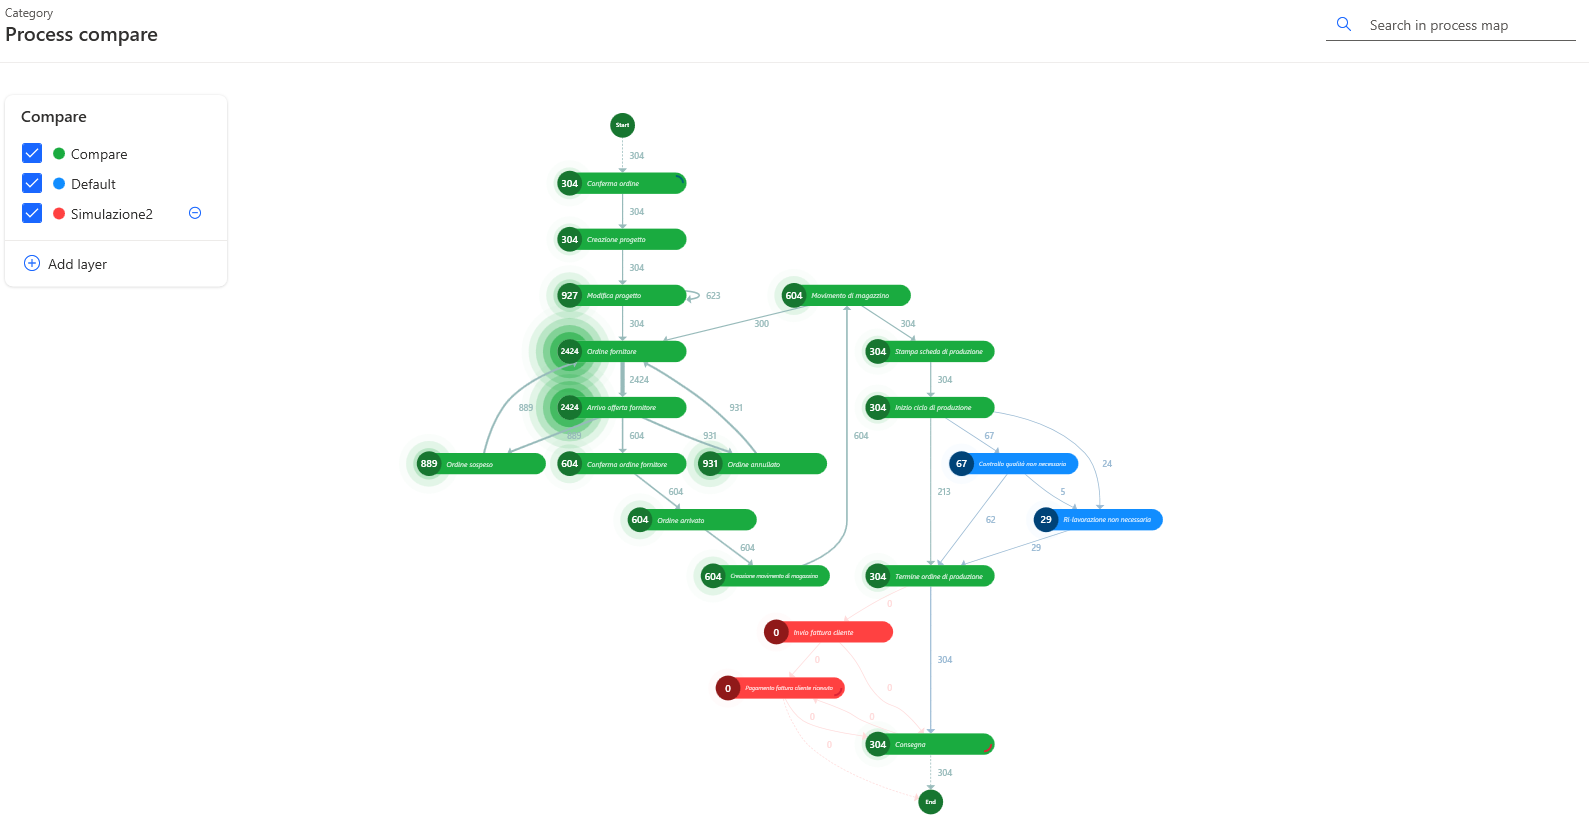
\includegraphics[width=\textwidth]{imgMicrosoft/TerzaSimulazione/ProcessComapareSimulazione3.png}
    \caption{Comparazione dei processi}
    \label{fig:process-compare}
\end{figure}
La funzionalità di comparazione dei processi rappresenta uno strumento particolarmente efficace all'interno delle soluzioni di process mining, poiché consente di mettere a confronto versioni diverse di un processo o varianti dello stesso flusso di lavoro. Grazie a questa funzionalità, è possibile visualizzare chiaramente le differenze tra i percorsi eseguiti, evidenziando i punti di divergenza e i tratti comuni tra i processi. Il vantaggio principale di questo strumento risiede nella sua capacità di mostrare graficamente come le attività siano distribuite e dove si verificano le principali discrepanze, utilizzando codici colore che rendono immediata la comprensione delle variazioni.\\
In particolare, la mappa di processo viene presentata con una codifica visiva che utilizza colori distinti per indicare le attività condivise e quelle uniche a ciascuna variante. Le attività comuni sono evidenziate in verde, mentre quelle esclusive di una specifica versione del processo appaiono in blu o in rosso. Questo approccio permette di identificare rapidamente dove i due processi seguono percorsi simili e dove, invece, si differenziano.\\
Un altro aspetto cruciale della funzionalità di comparazione è la stratificazione dei processi. Attraverso l’aggiunta di diversi strati, è possibile visualizzare simultaneamente più processi o varianti e osservare come questi interagiscano. Questo rende possibile sovrapporre le varianti del processo e vedere chiaramente le somiglianze e le differenze, fornendo una visione globale delle dinamiche operative.\\
La comparazione dei processi è essenziale non solo per monitorare i cambiamenti apportati a un processo esistente, ma anche per verificare se le modifiche implementate abbiano effettivamente prodotto i risultati desiderati. La possibilità di confrontare una nuova versione di un processo con quella precedente aiuta a valutare l'impatto di queste modifiche, permettendo di capire se il flusso sia stato ottimizzato o se siano emerse nuove problematiche. Allo stesso tempo, la funzionalità offre l’opportunità di standardizzare processi aziendali, specialmente in contesti dove è essenziale mantenere uniformità operativa tra diversi dipartimenti o sedi geografiche.\\

\section{Implementazioni pratiche: dati reali}
\end{document}